% Do not change the options here
\documentclass[bsc,frontabs,singlespacing,parskip,deptreport,normalheadings]{infthesis}

\usepackage{amsmath}
\usepackage{algorithm}
\usepackage{algpseudocode}
% https://qiita.com/sff1019/items/cb8cae96a1f7026656fc to get minted working with vimtex
\usepackage{minted}
\usemintedstyle{manni}
\usepackage[bookmarks=true]{hyperref}
\hypersetup{
    colorlinks=true,
    linkcolor=cyan,
}
\usepackage{bookmark}
\usepackage{quiver}

\begin{document}
\begin{preliminary}

\title{Need for Speed: Latency-Hiding Work-Stealing}

\author{Neil Weidinger}

% to choose your course
% please un-comment just one of the following
% \course{Artificial Intelligence}
%\course{Artificial Intelligence and Computer Science}
%\course{Artificial Intelligence and Mathematics}
%\course{Artificial Intelligence and Software Engineering}
%\course{Artificial Intelligence with Management}
%\course{Cognitive Science}
\course{Computer Science}
%\course{Computer Science and Management Science}
%\course{Computer Science and Mathematics}
%\course{Computer Science and Physics}
%\course{Computer Science with Management}
%\course{Software Engineering}
%\course{Software Engineering with Management}

\project{4th Year Project Report}

\date{\today}

\abstract{
This skeleton demonstrates how to use the \texttt{infthesis} style for
undergraduate dissertations in the School of Informatics. It also emphasises the
page limit, and that you must not deviate from the required style.
The file \texttt{skeleton.tex} generates this document and can be used as a
starting point for your thesis. The abstract should summarise your report and
fit in the space on the first page.
}

\maketitle

\section*{Acknowledgements}
Acknowledgements go here.

\tableofcontents

\end{preliminary}

%%%%%%%%%%%%%%%%%%%%%%%%%%%%%%%%%%%%%%%%%%%%%%%%%%%%%%%%%%%%%%%%%%%%%%%%%%%%%%%%

\chapter{Introduction}

This chapter provides a brief introduction and motivation to the problem of
latency-hiding work stealing, as well as the aims of this project. An outline of
the report is provided.

\section{Motivation}

Exploiting the parallel nature of modern processors is critical to achieving
high performance. In an era where even entry-level consumer tier hardware
features-shared memory parallelism, the need for software to be written that
makes efficient use of these resources is key to unlocking efficiency gains.
Unfortunately, the difficulty involved with the writing of parallel programs by
explicitly specifying which computations should map to which processor is
non-trivial and prone to introducing errors. Programmers need to manually
schedule computations and enforce synchronization using low-level primitives
such as locks and atomic operations, that are highly vulnerable to subtle and
non-deterministic errors like race conditions and deadlocking.

This backdrop of the need to embrace parallelism has spurred the advancement of
significant research and development in programming languages and paradigms to
help assist writing such programs \cite{muller_latency-hiding_2016,
zakian_concurrent_2016}. One such paradigm is \textit{\textbf{fork-join}}
parallelism \cite{conway_multiprocessor_1963, nyman_notes_2016}, where programs
can begin parallel execution at ``fork'' points and ``join'' to merge back and
resume sequential execution again. This alleviates the programmer from having to
manually managing parallel computation: one needs to only express the
\textbf{\textit{logical}} opportunities for \textit{\textbf{possible}}
parallelism, decoupling the programmer from the underlying runtime that takes
care of handling scheduling and execution.

Such an underlying runtime to manage parallelism while the program executes must
feature a \textit{\textbf{scheduler}} to determine an efficient parallel
execution. Runtime implementations such as Cilk
\cite{frigo_implementation_1998}, the Java Fork/Join framework
\cite{lea_java_2000}, and TBB \cite{noauthor_advanced_nodate}, commonly employ
\textbf{\textit{work-stealing}} \cite{blumofe_cilk_1995}: a class of schedulers designed to deal with the
problem of dynamically multithreaded computations on statically multithreaded
hardware. In brief, work-stealing schedulers take care
of scheduling and the accompanying issue of load balancing available work by
using a fixed pool of worker threads that are each responsible for maintaining a
local deque to keep track of this work. Worker threads execute work from the
bottom of their local deque, and when they run out of work they become
\textit{\textbf{thieves}} and \textit{\textbf{steal}} from the top of the deques
of other randomly selected worker threads.

Work-stealing has shown itself to be a very efficient approach to implementing
fork-join parallelism. Such schedulers have strong theoretical performance
guarantees \cite{blumofe_scheduling_1999} as well as proving themselves in
practice \cite{arora_thread_1998}. Research on work-stealing has proven fruitful
in the domain of traditional fine-grained parallelism, such as in
high-performance and scientific computing where workloads are dominated by
computational tasks: operations rarely incur latency and nearly all of the time
a processor spends executing an operation is useful work. General modern
workloads running on parallel architectures, however, frequently involve large
degrees of operations that do incur latency, commonly in the form of I/O:
waiting for user input, communicating to a remote client or server, dealing with
hardware peripherals, etc. In such environments, classic work-stealing
schedulers can suffer from large performance implications, depending on how much
latency is incurred while executing the workload
\cite{muller_latency-hiding_2016, singer_scheduling_2019, zakian_concurrent_2016}.

Classic work-stealing schedulers have no notion of latency-incurring operations
nor incorporate them into the design of the scheduling algorithm. A worker
thread that encounters a latency-incurring operation is
\textbf{\textit{blocked}}: it is performing no useful work, and is simply
wasting time waiting for the blocking operation to complete. Latency-incurring
operations cause underutilization of the available hardware resources,
potentially significantly impacting performance. An alternative to blocking
operations are to use \textbf{\textit{asynchronous}} (i.e. non-blocking) I/O
operations, but those come with their own set of challenges of managing
concurrent control flow \cite{niebler_structured_2020, smith_notes_nodate}.

Under such workloads, large performance gains can be made from having either the
latency-incurring operation cooperatively yield or the scheduler forcibly
preempting the operation, and allowing another task that could be performing
useful work to run instead. This allows the latency-incurring operation to wait
out its latency in the background even while all hardware resources are being
fully utilized on other tasks, thus \textbf{\textit{hiding}} the latency. Singer
et. al \cite{singer_proactive_2019}, introduce a latency-hiding work-stealing
scheduling algorithm, \textit{\textbf{ProWS}}, that utilizes
\textbf{\textit{futures}} (a parallel language construct
\cite{halstead_implementation_1984, halstead_multilisp_1985}) to represent and
schedule latency-incurring operations. Futures can be \textbf{\textit{spawned}}
to begin parallel execution, and return a handle future handle that can be
\textbf{\textit{touched}} (also commonly called \textbf{\textit{await}} or
\textbf{\textit{get}}) at a later point to retrieve the value of the operation.
ProWS, by proactively stealing whenever the scheduling algorithm encounters a
blocked future, can provide better bounds on execution time and other
performance metrics than previous work \cite{muller_latency-hiding_2016,
spoonhower_beyond_2009}.

Scheduling futures is only one part of the equation to fully support
latency-hiding work-stealing: a runtime system to efficiently dispatch and
process latency-incurring operations is also necessary. The use of futures to
hide latency is not much help if worker threads themselves must incur the cost
of awaiting futures; dedicated I/O threads and integration with operating system
event notification facilities is required. Singer et. al
\cite{singer_scheduling_2019} present an extension of Cilk, called Cilk-L, that
incorporates such runtime support with encouraging results.

TODO: better transition to talking about Rust

Rust \cite{matsakis_rust_2014} is a relatively new systems level programming
language aimed at delivering the low-level abilities and performance
characteristics of languages like C and C++, while ensuring far greater levels
of memory and thread safety. It achieves this by using a rich static type
system to allow the compiler to infer when and how values are safe to use,
termed the ``borrow checker''. It also has first class support for asynchronous
programming through the use of futures (futures in Rust have some idiosyncrasies
described in section \ref{section:futures}) and a quickly growing
ecosystem surrounding asynchronous programming in Rust. Rayon
\cite{noauthor_rayon_2022, noauthor_baby_nodate, stone_how_2021} is a
widely-used library level implementation for Rust programs (Cilk and its
derivatives consist of a both Cilk to C level compiler and a runtime library) of
work-stealing that supports task-level fork-join parallelism, but without
latency-hiding.

Futures in Rust, unlike the hand-written futures used in Cilk-L, are easily
composable: the compiler automatically generates a state machine that represents
the current state of an asynchronous operation. This allows for ergonomic
user-defined asynchronous operations that highly resemble regular sequential
code, and powerful future combinators \cite{noauthor_futuresfuture_nodate}.
Supporting this behavior requires a few additional capabilities than what ProWS
provides directly.

\section{Aims}

The aim of this project is to provide an implementation, building heavily upon
the work of Singer et. al, of latency-hiding work-stealing that seamlessly
integrates with the Rust language and ecosystem.

This report describes the
design, implementation, and evaluation of ProWS-R, a variant of ProWS that is
adapted for the particular futures found in Rust and its stringent safety
guarantees.

This report describes ProWS-R, a variant of ProWS that is adapted for the
particular futures found in Rust, as well as taking careful consideration with
regards to the stringent safety guarantees and ergonomics of the language. The
accompanying runtime library Rayon-LH, a fork of the Rayon library, is also
presented. The design, implementation and subsequent evaluation of ProWS-R are
???

The explicit goals of this project are as follows:

\begin{itemize}
    \item TODO: explicit goals
    \item Present a latency-hiding work-stealing algorithm, that takes
        accommodates the language-level futures construct in Rust
    \item Develop a prototype implementation of 
\end{itemize}

\section{Contributions}

\section{Report Outline}

%%%%%%%%%%%%%%%%%%%%%%%%%%%%%%%%%%%%%%%%%%%%%%%%%%%%%%%%%%%%%%%%%%%%%%%%%%%%%%%%

\chapter{Background: What Andy Giveth, Bill Taketh}

Describe and outline background chapter.

\section{Modern Computer Architecture}

Ever since the advent of general-purpose microprocessor based computer systems,
transistor density has been and continues to double roughly every two years.
Famously known as Moore's law, for the first 30 years of the existence of the
microprocessor the consequences of this graced the computing world with
effortless biennial performance increases. Bestowed with this exponential growth
of transistor density, chip designers could drastically increase core
frequencies with each generation, and with ever increasing transistor budgets
afford to design more complex architectural features like instruction
pipelining, superscalar execution, and branch prediction. Without touching a
line of code, software developers could expect programs to automatically double
in performance every two years \cite{hennessy_new_2019}.

Accompanying Moore's law was another, related, effect: Dennard scaling. While
Moore's law provides increased transistor counts, Dennard scaling allowed for
this transistor doubling while ensuring power density was constant. The scaling
law states roughly that as transistors get smaller, power density stays
constant, meaning that power consumption with double the transistors stays the
same. Additionally, as transistor sizes scale downward, the reduced physical
distances enable reduced circuit delays, meaning an increase in clock frequency,
boosting chip performance. When combined, with every technology generation
transistor densities double, clock speeds increase by roughly 40\%, and power
consumption remains the same \cite{borkar_future_2011}. This remarkable scaling
is what historically allowed for incredible performance gains year over year,
all while keeping a reasonable energy envelope.

But starting around 2005, Dennard scaling has broken down: processors have
reached the physical limits of power consumption in order to avoid thermal
runaway effects that would require prohibitive cooling solutions (CPU chips that
would melt would likely be difficult to sell to customers). This is known as the
power wall, and chip designers could no longer regularly rely on increasing
clock frequencies to deliver performance gains \cite{parkhurst_single_2006}. The
multicore era was born.

\subsection{Rise of the Multicore Era}

While the doubling of transistor count observation of Moore's law is still going
strong, the historic predictable free performance lunch it became associated
with is no longer what is once was. Instead of being dedicated to more complex
architectural features in order to extract sequential performance on single core
processors, the extra transistors are largely used to build more cores on a
single processor. With diminishing returns on effort spent increasing single
core performance, chip designers look to add multiple cores to be able to
execute more instructions in parallel \cite{patterson_trouble_2010}.

CPU performance can be described using the following equation
\cite{patterson_computer_2021}, where performance is measured in terms of
absolute execution time: \[ \text{CPU execution time for a program} =
\frac{\text{Program instruction count} \cdot \text{CPI}}{\text{Clock rate
(frequency)}} \]

where CPI is average clock cycles per instruction. No longer able to increase
the clock frequency due to the power wall and increasing difficulty reducing
CPI, efforts of hardware architects focused on simply reducing program
instruction count per processor, by distributing instructions across multiple
CPU cores to be executed in parallel \cite{etiemble_45-year_2018}.

Multicore processors are microprocessors containing multiple processors in a
single integrated circuit, where each of these processors is known as a core.
Almost all commodity multicore processors today are \textit{symmetric
multiprocessing (SMP)} systems, meaning all cores in a processor share the same
physical address space. A single physical address space allows cores to operate
on shared data.

Armed with multiple cores, different programs or different parts
of the same program can be run at the same time in parallel, reducing the time
required to perform the same amount of work on a single processor, boosting
performance. No longer limited to a single processor core executing work,
programs stand to drastically benefit in execution throughput by being run on
multiple cores simultaneously.

As of 2021, it is difficult to find a processor that is not a multicore
processor. The performance gains provided by having multiple cores have shown to
be so profound that even the lowest end chips feature multiple cores. The
Raspberry Pi Zero 2, a \pounds13.50 board in the Raspberry Pi family of low cost
single-board computers, features a 64-bit quad-core Arm Cortex-A53 CPU
\cite{ltd_raspberry_nodate}.

Initially, multicore processors may seem like a silver bullet to the question of
what to do when faced with the power wall: for more performance, simply scale
the number of cores! In reality, as is typical, the situation is more nuanced.
Many workloads cannot be trivially diced up and processed on multiple cores, and
even if so, support for splitting up work and then computing this work in
parallel must be explicitly supported and designed for.

\subsection{Parallel Computing and its Difficulties}
\label{section:parallel_computing}

Although multiple cores on a single chip running in parallel offer tantalizing
performance benefits, there is one catch: programmers must write explicitly
parallel programs. Software must be carefully designed such that it actually
takes advantage of multiple processing units: a single-threaded application
running on an 8 core CPU can only take advantage of 1/8 of such a chips
potential throughput. Worst of all, after about nearly two decades of experience
since the introduction of the first multicore processors, experience has shown
that compared to traditional sequential programming, parallel programming is
simply very difficult \cite{creeger_multicore_2005, lee_problem_2006,
patterson_trouble_2010}.

\begin{itemize}
    % TODO
    \item There are many things a programmer must be aware of when writing
        parallel programs (\textbf{CONDENSE})
    \begin{itemize}
        \item Synchronization of memory accesses
        \item Synchronization of control flow
        \item Memory ordering
        \item Race conditions
        \item Deadlocks/livelocks
        \item Lock-free programming and atomic operations
        \item Workload partitioning
        \item Workload balancing
        \item Scheduling
    \end{itemize}
\end{itemize}

Before the introduction of mainstream multicore processors, code was written
with the intention of being executed in serial on a single core processor. Once
CPU hardware started featuring multiple cores, programs did not magically
rewrite themselves to take advantage of this increased firepower. Instead,
developers had to manually identify the existing parallelism in their programs
and refactor them to run as multiple computational threads
\cite{patterson_trouble_2010}.

Threads are an abstraction of units of scheduling and execution: the same
program can have multiple threads of execution running concurrently. A
\textit{\textbf{thread scheduler}} manages these threads \footnote{Typical thread
    schedulers however have no knowledge of the thread workloads; all threads
    are opaque to the scheduler: the scheduler does not know whether a given
    thread has operations that must complete before operations in another
    thread, the scheduler simply chooses a thread to run according to its
scheduling algorithm (that typically tries to schedule all threads
fairly/evenly) and it is up to the programmer to explicitly program this thread
synchronization.} and chooses when they should run on the CPU. Multicore
processors allow threads to truly run in parallel, instead of just concurrently
as would happen on a single core processor, as multiple cores can each be
executing a thread simultaneously.

Threads are the most common approach to concurrent programming and by extension
parallel programming, but are notoriously difficult to use efficiently and
and ensure correctness with \cite{lee_problem_2006}.

Other approaches to parallel computing, for example network connected cluster
based designs frequently found in the high performance computing (HPC) domain,
will not be discussed in this report, although the ideas described could
possibly be transferable.

Not only does software need to be written with the above concepts in mind, there
is an inherent limit to how much a given program can even take advantage of the
parallelism offered by multiple processors. Not all program can benefit from
being run in parallel, and those that do have their maximum theoretical speedups
capped by Amdahl's Law.

% TODO
\subsection{Amdahl's Law (REMOVE)}

Amdahl's law provides an upper bound to the potential speedup a program can
benefit from when the performance of a portion of the program is improved, and
is often used in parallel computing to predict the maximum theoretical speedup
when using multiple processors. A program that required \(T_\text{old}\) time to
execute that now has a fraction \(\alpha\) of it running in parallel on \(k\)
processors has a theoretical speedup \(S = T_\text{old} / T_\text{new}\) of \[ S
= \frac{1}{(1 - \alpha) + \alpha / k} \]

A derivation can be found in \cite{bryant_computer_2016}. If we consider setting
\(k\) to \(\infty\), we can see the maximum possible speedup \(S_\infty\) of a
program running on an infinite number of processors is \(1 / (1 - \alpha)\). The
major insight of Amdahl's law is that to speed up the entire program, the speed
of a very large fraction of the program must be significantly improved, and even
then there is an upper bound on the possible speedup that can be achieved. In
other words, a program that wishes to take advantage of being run in parallel
must exhibit an ample amount of parallelism (fraction of the program that can be
run in parallel) to demonstrate an advantage when compared to running on a
single processor.

\section{Classical work stealing}

\subsection{Motivating Examples}

\begin{itemize}
    \item Fibonacci example for compute bound
    \item Include latency-incurring example here in BG chapter, or later?
\end{itemize}

\subsection{DAG model of Parallel Computations}

\begin{itemize}
    \item Taken largely from \cite{cormen_introduction_2009, herlihy_art_2012,
        blumofe_executing_1995}
    \item With typical sequential computing, all instructions can be defined as
        a totally ordered set of instructions, where the ordering specifies the
        execution order. With multithreaded computing, a computation can be
        defined as a partially ordered set of instructions, which may be
        executed in any order that complies with the partial ordering.
    \item This partial ordering in a multithreaded computation can be
        represented as a DAG \(G = (V, E)\)
    \item Each node in \(V\) represents an instruction to be executed
    \item Each directed edge in \(E\) represents dependencies between
        instructions
    \begin{itemize}
        \item Edge \((u,v) \in E\) means that instruction \(u\) must execute
            before instruction \(v\)
        \item A horizontal edge, called \textbf{continuation} edges, represents
            the sequential ordering in a given thread (threads are the
            horizontal shaded blocks of sequential instructions)
        \item A thread can spawn another thread, which is indicated by a
            downward edge originating from a \textbf{spawn instruction}. Spawn
            instructions, the instruction that actually performs the spawn
            operation, are the only nodes with outdegree of 2. Spawns introduce
            parallelism: instructions in different threads can execute
            concurrently, and by extension execute in parallel.
        \item An upward edge, called a \textbf{join edge}, represents points of
            synchronization: instruction nodes that have incoming join edges
            wait until all previous instructions have executed before
            proceeding.
    \end{itemize}
    \item If a directed path exists between \(u\) and \(v\), they are
        (logically) in series, and execute serially just like in typical
        serial programs (doesn't say anything about when they're executed,
        only that they must not execute in parallel and must execute in
        order specified)
    \item Otherwise if a path does not exist, they are (logically) in
        parallel, meaning they \textit{\textbf{may}} execute in parallel (does not specify
        that they \textit{\textbf{will}} execute in parallel, only that at runtime a
        scheduler is allowed to choose to run them in parallel by assigning
        them to available processors)
\end{itemize}

\subsection{Analysis of Parallel Computations}
\label{subsection:analysis_of_parallel_computations}

\begin{itemize}
    \item To analyze the theoretical performance of multithreaded program, we
        need a more formal way of describing the efficiency of such programs
    \item Let \(T_P\) be the running time of a multithreaded program run on
        \(P\) processors
    \item The \textbf{work} of a computation is the total time required to
        execute each computation node in the DAG. In other words, work is the
        time required to execute the computation on a single processor: \(T_1\).
    \item The \textbf{span} (also called critical path) of a computation is the
        length of the longest sequence of computations that need to be executed
        serially, due to computation dependencies represented as edges in the
        DAG. In other words, the span is the running time if the computation
        could be run on an infinite number of processors, denoted by
        \(T_\infty\).
    \item Ideally, to reduce execution time, a computation minimizes the work
        and span
    \item Using the above two definitions, we arrive at two very useful results:
    \begin{itemize}
        \item \textbf{Work law:} Since \(P\) processors can perform at most
            \(P\) operations in one time step, the total amount of work
            performed in \(T_P\) time is \(P T_P\). Since the total amount of
            work to be done is \(T_1\), we see that \[P T_P \geq T_1\] This can
            also be interpreted as the fact that the time \(T_P\) to run the
            computation on \(P\) processors is at least the time taken to run on
            one processor \(T_1\) divided by the number of processors \(P\):
            \[T_P \geq T_1 / P\]
        \item \textbf{Span law:} Since the time taken to run a computation on a
            finite number of processors \(P\) cannot be faster than the time
            taken on an infinite number of processors, we have \[T_P \geq
            T_\infty\]
    \end{itemize}
    \item Now we can define a few useful performance metrics:
    \begin{itemize}
        \item \textbf{Speedup:} Defined by the ratio \(S_P = T_1 / T_P\),
            expressing how much faster the computation is on \(P\) processors
            than on 1 processor. Rearranging the work law, we see that \(T_1 /
            T_P \leq P\), meaning that the speedup gained by running on \(P\)
            processors is at most \(P\). When the speedup scales linearly
            with the number of processors \(T_1 / T_P = \Theta(P)\), we have
            \textit{\textbf{linear speedup}}, and when \(T_1 / T_P = P\) we have
            \textit{\textbf{perfect linear speedup}}.
        \item \textbf{Parallelism:} The amount of \textit{\textbf{parallelism}} in a
            computation is expressed by the ratio \(T_1 / T_\infty\). This
            represents the average number of computations that can be performed
            in parallel at \textit{\textbf{each step}} along the critical path. This is
            also the maximum possible speedup that can be achieved on any number
            of processors (using the span law: \(T_1 / T_P \leq T_1 /
            T_\infty\)). We see that there is not much point in using
            \(P\) processors when \(P > T_1 / T_\infty\), as the extra
            processors will just be idle not performing work.
    \end{itemize}
\end{itemize}

\subsection{Scheduling}

\begin{itemize}
    \item Our model of multithreaded computation does not specify which
        instructions to run on which processors at what point in time: this is
        the job of the \textbf{scheduler}.
    \item A scheduler constructs an \textbf{execution schedule} that maps
        instruction nodes in the multithreaded computation DAG to processors at
        each step in time \footnote{In practice, our scheduler that breaks down
            the multithreaded DAG is a user-space scheduler that maps
            instructions on to threads (as many as there are processors), and an
            operating system level thread scheduler then schedules these OS
            level threads. In other words, a userspace scheduler maps
        instruction nodes onto a fixed number of OS threads, and the kernel
    level scheduler maps these threads onto hardware processor cores.}. A
    typical goal for a scheduler is to reduce absolute execution time (we later
    prove asymptotic bounds for our scheduler in terms of the work and span). At
    any given point in time a processor is either active or idle; a scheduler
    tries to minimize the amount of time a processor sits idle.
    \item An execution schedule must satisfy all constraints given
    by the edges
        present in the DAG, such that the partial ordering of instructions is
        satisfied.
    \item As mentioned in section \ref{section:parallel_computing}, programmers
        can themselves schedule when threads in their programs should be run as
        well as ensure proper synchronization. This low-level manual thread
        orchestration, however, becomes increasingly difficult with the number
        of threads involved, especially when shared resources and thread
        synchronization are required: the sheer number of possible interleavings
        of code execution quickly becomes unwieldy. Not only are threads
        difficult to reason about conceptually, it is also important for the
        programmer to perform efficient load balancing of processors to optimize
        utilization of available computing resources. A programmer would have to
        manually use complex communication protocols to ensure each thread
        receives a balanced amount of work to execute, which can be difficult
        and error prone.
    \item An easier approach is to raise the level of abstraction, and instead
        only require programmers to merely \textit{\textbf{expose}} sections of possible
        parallelism in their programs, while letting a runtime system take care
        of the thread creation and building an execution schedule. The runtime
        systems in turn then becomes responsible for such a schedule that not
        only satisfies all ordering constraints, but also achieves high
        performance and efficiency.
\end{itemize}

\subsection{Work Stealing}
\label{subsection:work_stealing}

\section{Futures}
\label{section:futures}

TODO: put general stuff about futures concept here

\subsection{Futures in Rust}
\label{subsection:futures_in_rust}

TODO: describe how futures in Rust work here (e.g. state machine, async fns,
executors, pinning, etc.)

\subsection{Futures and DAGs}

A diagram of a (partial) DAG for the distributed map and reduce example is shown
in figure \ref{fig:map-reduce-dag}. The bolded red lines represent edges in the
DAG that incur latency of the network request, that is simulated in the
benchmark with a simple future that suspends for a desired duration. Without
latency-hiding, \textit{each} of the latency-incurring edges must be incurred by
the worker threads, while with (perfect) latency-hiding just the cost of the
\textit{single} heaviest latency-incurring edge on the critical path is
incurred. TODO: move this figure and explanation to the background, would
provide a nice introduction and subsequent conclusion here

\begin{figure}[ht]
    \centering
    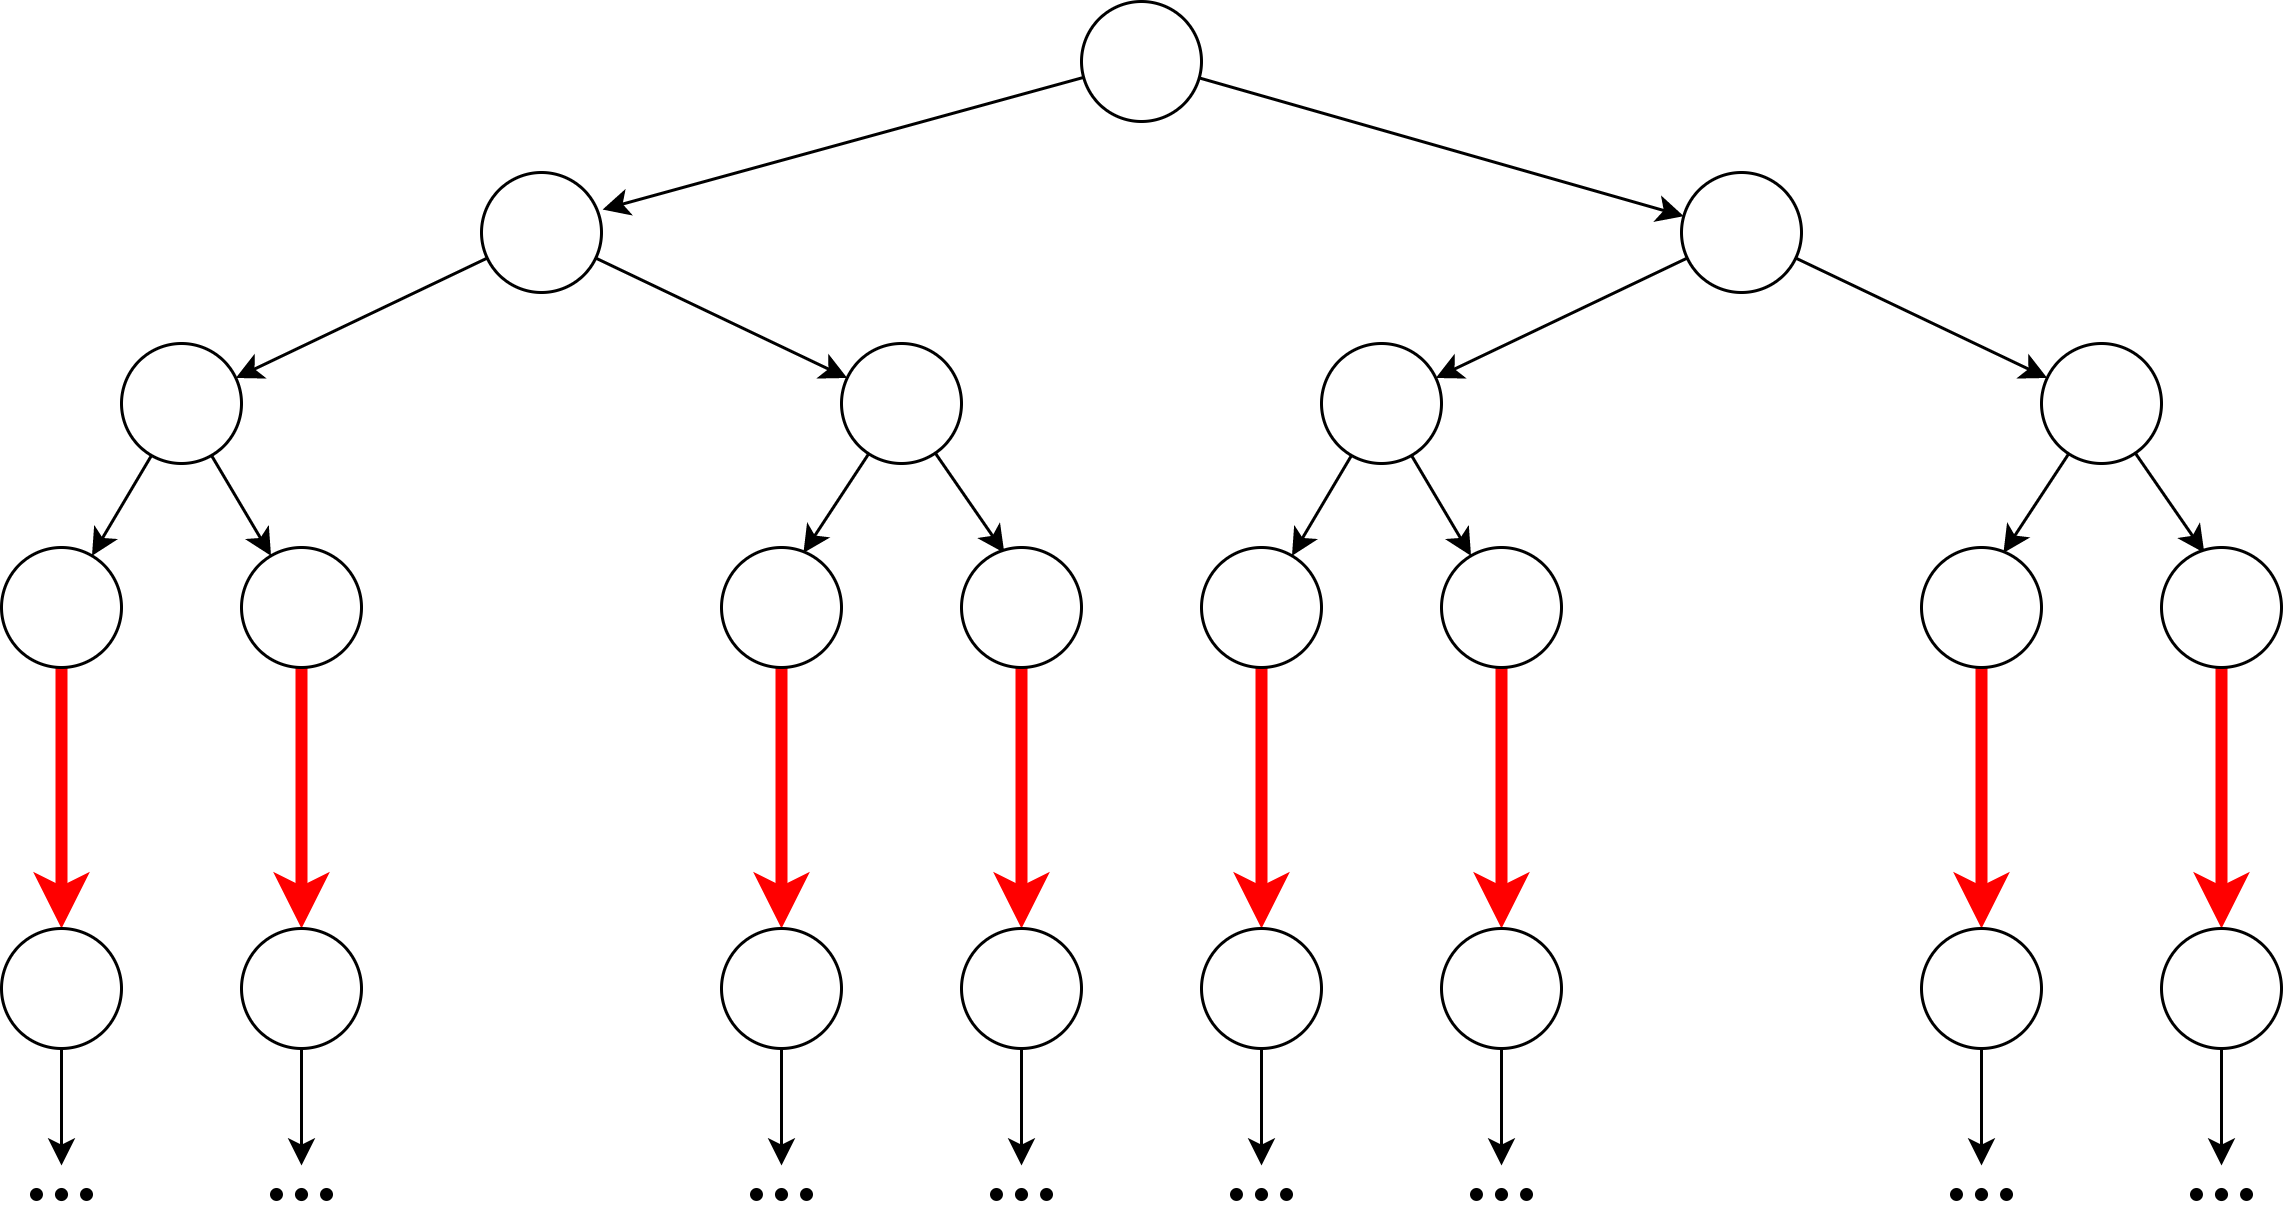
\includegraphics[width=0.6\textwidth]{figures/map-reduce.png}
    \caption{A partial DAG for map and reduce}
    \label{fig:map-reduce-dag}
\end{figure}

TODO: describe how futures can be incorporated into analysis of parallel
computations using DAG model

\section{Survey of Related Work}

%%%%%%%%%%%%%%%%%%%%%%%%%%%%%%%%%%%%%%%%%%%%%%%%%%%%%%%%%%%%%%%%%%%%%%%%%%%%%%%%

\chapter{Conceptual Latency-Hiding: To Wait Or Not to Wait?}
\label{chapter:conceptual_latency-hiding:_to_wait_or_not_to_wait?}

This chapter describes the high-level overview of the ProWS-R latency-hiding
work stealing algorithm, without diving into the details of the implementation.
Section \ref{section:overview_of_the_prows_algorithm} provides an overview of
the core scheduling algorithm, and the considerations that allow for repeatedly
polled futures found in Rust. Section
\ref{section:required_runtime_support_for_latency_hiding} describes the
additional runtime support necessary to provide the latency-hiding capabilities
of the scheduler.


\section{The ProWS-R Algorithm}
\label{section:overview_of_the_prows_algorithm}

This section is heavily based on the work done in \cite{singer_proactive_2019},
where the authors introduce the ProWS scheduling algorithm. ProWS is a provably
efficient algorithm that introduces support for the generalized concept of
futures, that deviates from traditional work-stealing algorithms by being
\textit{\textbf{proactive}}, detailed in section 
\ref{subsection:parsimonious_vs_proactive_work-stealing}. Presented here is an
exposition of the ProWS-R algorithm, a variant of ProWS, with details on the
considerations taken to support the Rust implementation of futures.

\subsection{Parsimonious vs Proactive Work-Stealing}
\label{subsection:parsimonious_vs_proactive_work-stealing}

Before jumping into the core algorithm, it's insightful to touch upon the
differences between parsimonious and proactive work-stealing. The consequences
of this mainly affect the theoretical execution bound (section
\ref{subsection:performance_bounds}) and on the number of
\textit{\textbf{deviations}} \cite{spoonhower_beyond_2009}, a metric used to
analyze the theoretical performance of parallel executions. Informally, the
difference between a parsimonious and proactive work-stealing scheduler boil
down to what actions are taken upon encountering a blocked future: a
parsimonious scheduler continues execution by popping nodes off its worker
deque, while a proactive scheduler opts to immediately become a thief and
attempts to steal work from elsewhere. 

The classic work-stealing scheduler, as described in section
\ref{subsection:work_stealing}, is parsimonious. Given the online scheduling
problem where the computational DAG unfolds as execution proceeds, it is the
responsibility of the scheduler to map work to available processing resources in
a way that is efficient and still preserves the sequential dependencies of nodes
in the DAG. Parsimonious scheduling achieves this by having each worker thread
maintain its own deque of nodes that represent work to be executed, and having
workers continuously pops nodes off and executing them. Upon completion of a
node execution, the node may enable zero, one, or two child nodes. If zero nodes
are enabled, it attempts to pop off its deque. If one node is enabled, it
immediately executes the enabled node. If two nodes are enabled, it pushes one
of the nodes to its end of the deque and executes the other.

Only when a worker runs out of work, signified by its deque being empty, does it
attempt to steal work from another worker. It becomes a thief and randomly
selects a victim deque, attempting to pop off a node from the top. Crucially, in
the context of dealing with futures, a blocked future simply falls under the
case of zero nodes, meaning a worker continues looking for work in its local
deque. The scheduler presented by Muller and Acar
\cite{muller_latency-hiding_2016} is such an algorithm: upon encountering a
blocked future, it sets the suspended future to the side but continues executing
nodes from its deque.

In contrast, the defining characteristic of proactive work-stealing is what
occurs instead upon encountering a blocked future: the deque is suspended and
the worker immediately attempts to find work elsewhere, by becoming a thief. In
ProWS-R, a worker marks its current deque (that it popped the future off of) as
\textbf{\textit{suspended}}, randomly selects another worker to assign this
suspended deque to, and then tries to steal work from other workers.
Importantly, this means that although there are \(P\) workers, there can be more
than \(P\) deques at a given time. Although it may initially appear
counterintuitive to proactively steal, as it may seem to increase the amount of
steal attempts and corresponding scheduler overhead, but doing so provides a
better bound on execution time given latency-incurring operations (section
\ref{subsection:performance_bounds}).

\subsection{Algorithm Overview}
\label{subsection:the_algorithm_in_detail}

Presented here is a description of the ProWS-R algorithm, the conceptual data
structures used, and the adjustments made to accommodate the futures found in
Rust. Again, this is largely based upon the work of Singer et. al, and their
work should be consulted as reference.

The principle idea behind ProWS-R is that there can be multiple deques in the
system at any given time, and each worker thread owns an \textbf{\textit{active
deque}} that they work off of. Whenever a worker thread encounters a blocked
future, its current active deque is marked as suspended, the worker relinquishes
ownership of the deque, and it attempts to find work elsewhere. The act of
suspending deques allows for the latency of latency-incurring operations to be
hidden while worker threads can fully utilize the available hardware resources
to make progress on remaining available work. This differs from classic
work-stealing, where such a scheduler without even the concept of
latency-incurring operations would simply treat the operation as a regular
computation, and be forced to block until the latency is incurred. When a worker
thread is executing a node and does not encounter a blocked future, the
algorithm proceeds the same as classic work stealing.

When a blocked future reaches completion, a callback is executed that marks the
deque as \textbf{\textit{Resumable}}, indicating that the previously suspended
deque now has work available and is free to have its work stolen by worker
threads. Worker threads have the ability to either steal just the top node off
of other deques (including the active deques of other workers), or
\textit{\textbf{mug}} entire deques that are marked as Resumable (but are not
the active deques of other workers), and claim ownership of such deques. Mugging
allows for the entire deque to be stolen in one go, as opposed to workers having
to repeatedly steal nodes one-by-one off of such deques (since they're not the
active deques of any other workers). 

\subsection{Data Structures}

\subsubsection*{Deques}
\label{subsubsection:deques}

Like in classic work-stealing, nodes that represent work in the computational
DAG are stored in deques. Deques are assumed to have support for concurrent
operations. Each worker thread owns an active deque that they pop nodes off the
bottom of and execute, like in classic work-stealing. If nodes spawn child
nodes, these are pushed to the bottom of the deque. Worker threads, when
stealing, pop nodes off the top of these deques. Worker threads also have the
ability to steal entire deques at once (called mugging) that then become the new
designated active deque for the respective worker thread. Each worker thread, in
addition to having an active deque, manages a set of \textbf{\textit{stealable}}
deques, called a \textbf{\textit{stealable set}}, that are not being actively
worked on but contain ready nodes that can be stolen and executed. Deque
operations are assumed to take constant amortized time.

Deques support the following operations:

\begin{itemize}
    \item \texttt{popTop}: pop top node off of deque
    \item \texttt{popBottom}: pop bottom node off of deque
    \item \texttt{pushBottom}: push node to bottom of deque
    \item \texttt{isEmpty}: return true if there are no nodes in deque
    \item \texttt{inStealableSet}: return true if this deque is to be found in a
        worker thread's stealable set
\end{itemize}

During execution of the algorithm, deques are in one of the following states:

\begin{itemize}
    \item \textbf{Active}: It is the designated active deque of a given worker
        thread (the worker thread treats this as its local deque).
    \item \textbf{Suspended:} The bottom-most node that was last executed by a
        worker thread encountered a blocking operation, and is now waiting out
        the latency of the operation. This node is \textit{not} in the deque; it
        will later be pushed onto the deque again by a callback when the
        operation completes. The deque may still contain other ready nodes that
        are available for worker threads to steal. TODO: make sure ``ready''
        nodes is defined
    \item \textbf{Resumable:} All nodes in the deque are ready, but is not being
        actively worked on by a worker thread. These nodes can be stolen off the
        top of the deque by worker threads and then executed.
    \item \textbf{Muggable:} The entire deque can be mugged by a worker thread,
        to become the threads new active deque.
\end{itemize}

\begin{figure}[ht]
% https://q.uiver.app/?q=WzAsNCxbMCwwLCJcXHRleHR7QWN0aXZlfSJdLFs1LDMsIlxcdGV4dHtSZXN1bWFibGV9Il0sWzUsMCwiXFx0ZXh0e1N1c3BlbmRlZH0iXSxbMCwzLCJcXHRleHR7TXVnZ2FibGV9Il0sWzAsMiwiXFx0ZXh0e0VuY291bnRlciBibG9ja2VkIGZ1dHVyZX0iLDFdLFsyLDEsIlxcdGV4dHtDb21wbGV0aW9uIG9mIGJsb2NrZWQgZnV0dXJlfSIsMV0sWzEsMywiXFx0ZXh0e1N0b2xlbiBieSB0aGllZiBvbmNlIGJlZm9yZX0iLDFdLFszLDAsIlxcdGV4dHtNdWdnZWQgYnkgdGhpZWZ9IiwxXV0=
\[\begin{tikzcd}
	{\text{Active}} &&&&& {\text{Suspended}} \\
	\\
	\\
	{\text{Muggable}} &&&&& {\text{Resumable}}
	\arrow["{\text{Encounter blocked future}}"{description}, from=1-1, to=1-6]
	\arrow["{\text{Completion of blocked future}}"{description}, from=1-6, to=4-6]
	\arrow["{\text{Stolen by thief once before}}"{description}, from=4-6, to=4-1]
	\arrow["{\text{Mugged by thief}}"{description}, from=4-1, to=1-1]
\end{tikzcd}\]
\caption{Deque state transitions}
\label{figure:deque_state_transitions}
\end{figure}

Deque transitions are displayed in figure \ref{figure:deque_state_transitions}.
Deques begin their lives in the Active state, when they are first created by a
worker thread. A worker thread then works off the bottom of this deque, until it
encounters a blocked future node, at which point the deque becomes Suspended.
Upon completion of the previously blocked future node, a callback is executed
that transitions the deque into the Resumable state. At this point, any worker
thread is able to steal a single node off the top of the deque. After a worker
thread has stolen a node off the top, the deque transitions into the Muggable
state. In this state a worker thread can steal the entire deque at once (a
mugging), and become the worker thread's new active deque.

\subsubsection*{Stealable Sets}
\label{subsubsection:stealable_sets}

In order to keep track of stealable deques, each worker thread owns a
\textbf{\textit{stealable set}}. This set contains deques that have ready nodes
that are ready to be executed (i.e. available work for worker threads to
perform). Like deques, stealable sets are assumed to support concurrent
operation and take constant amortized time. During scheduler execution, thieves
select a victim worker thread uniformly at random to steal from, and from within
that victim's stealable set, uniformly at random select a victim deque.

Stealable sets support the following operations:

\begin{itemize}
    \item \texttt{add}: add a deque to the set
    \item \texttt{remove}: remove a deque from the set
    \item \texttt{chooseRandom}: return a random deque from the set (without
        removing it)
\end{itemize}

\subsection{Scheduling Loop}

The main scheduling loop is shown in algorithm \ref{alg:scheduling_loop}.
Execution starts by setting the active deque of all worker threads to an empty
deque, and pushing the root of the computation to one of the deques, after which
the scheduling loop begins (line \ref{line:loop}).
Without the extra logic to deal with futures (lines \ref{line:future_start} -
\ref{line:future_end}), ProWS-R behaves the same as classic work-stealing.

\begin{algorithm}
\caption{Main Scheduling Loop ($w$ is the currently executing worker thread)}
\label{alg:scheduling_loop}
\begin{algorithmic}[1]
    \Function{schedulingLoop}{}
        \While{computation is not done} \label{line:loop}
            \State $node \gets \text{findNode()}$
            \State $left, right \gets \text{execute(}node\text{)}$
            \If{$left \neq \text{null}$}
                \State $w \text{.active.pushBottom(}left\text{)}$
            \EndIf
            \If{$right \neq \text{null}$}
                \State $w \text{.active.pushBottom(}right\text{)}$
            \EndIf
            \If{$node \text{ encountered blocked future } f$}
            \label{line:future_start} \label{line:blocked_future}
                \State $deq \gets w \text{.active}$
                \State $w \text{.active} \gets \text{null}$
                \State $\text{suspendDeque(}deq\text{)}$
                \State $f\text{.installCallBack(} deq \text{)}$
                    \label{line:install_callback}
            \EndIf \label{line:future_end}
        \EndWhile
    \EndFunction
    \algstore{loop}
\end{algorithmic}
\end{algorithm}

\begin{algorithm}
\caption{Find Node ($w$ is the currently executing worker thread)}
\label{alg:find_node}
\begin{algorithmic}[1]
    \algrestore{loop}
    \Function{findNode}{}
        \State $node \gets \text{null}$
        \If{$w \text{.active} \neq \text{null}$}
            \State $node \gets w \text{.active.popBottom()}$
        \EndIf
        \If{$node = \text{null}$} \label{line:no_work}
            \State $node \gets \text{steal()}$
        \EndIf
        \State $\textbf{return} node$
    \EndFunction
    \algstore{findnode}
\end{algorithmic}
\end{algorithm}

Worker threads work off the bottom of their active deques. When a node is popped
from the bottom, it is first executed and then its children (if any) are pushed
to the bottom of the deque. Special care is taken for when a node that was just
executed is found to have encountered a blocked future (line
\ref{line:blocked_future}): the worker thread's active deque is immediately
suspended and a callback is installed on the future that will reschedule it for
execution again once it's latency-incurring operation completes. Deque
suspension for the active deque (line \ref{line:deque_suspension}) involves
changing its state to Suspended, removing it from the worker thread's stealable
set, and if it is not empty, adding it to the stealable set of another randomly
selected worker thread. If the deque is empty, it will not be found in any
stealable set, so that worker threads can not try to fruitlessly steal from it. 

\begin{algorithm}
\caption{Deque Suspension ($w$ is the currently executing worker thread)}
\label{alg:suspend_and_find}
\begin{algorithmic}[1]
    \algrestore{findnode}
    \Function{suspendDeque}{$deq$} \label{line:deque_suspension}
        \State $deq\text{.state} \gets \textbf{SUSPENDED}$
        \State $ w \text{.stealableSet.remove(} deq \text{)}$
        \If{$! deq \text{.isEmpty()}$}
            \State $ \text{chooseRandomVictim().stealableSet.add(} deq \text{)}$
        \EndIf
    \EndFunction
    \algstore{suspend}
\end{algorithmic}
\end{algorithm}

The callback (line \ref{line:callback}) that is installed on the blocked future
(line \ref{line:install_callback}) is the critical aspect for enabling
latency-hiding. In order to try and keep worker threads busy with work as much
as possible so that progress is being made on the computation with full hardware
resource utilization, it's undesirable for worker threads to perform any
operations that are not directly related to executing work nodes (contributes to
scheduler overhead). As such, the callback is responsible for executing when
completion of a blocked future is detected, and rescheduling the future node for
execution by a worker thread. A more concrete reasoning and explanation of how
this occurs is given in section
\ref{section:required_runtime_support_for_latency_hiding}.

\begin{algorithm}
\caption{Callback Procedure (called upon completion of the blocked future $f$)}
\label{alg:callback}
\begin{algorithmic}[1]
    \algrestore{suspend}
    \Function{callBack}{$suspendedDeq$} \label{line:callback}
        \If{$suspendedDeq \text{.state} \neq \textbf{SUSPENDED} $}
            \label{line:sus_check}
            \State \textbf{return}
        \EndIf
        \State $suspendedDeq \text{.pushBottom(} f \text{)}$ \Comment $f$ is a node
            that can be executed
        \State $suspendedDeq\text{.state} \gets \textbf{RESUMABLE}$
        \If{$! suspendedDeq \text{.inStealableSet()}$}
            \State $\text{chooseRandomVictim().stealableSet.add(} suspendedDeq
                \text{)}$
        \EndIf
    \EndFunction
    \algstore{callback}
\end{algorithmic}
\end{algorithm}

Due to the way Rust futures implement their completion signaling mechanism using
wakers (introduced in section \ref{subsection:futures_in_rust}), it is possible
for multiple wakers to wake up the same future. This is unlike the futures
supported by ProWS, and it is vital that ProWS-R take specific care to handle
\textit{repeatedly polled futures}. Multiple polled futures can happen, for
example, when two futures are manually polled immediately after one another
using the same waker, like when using the \texttt{join} function \footnote{The
    \texttt{join} function in the Rust futures crate \footnote{Crates in Rust
    are essentially synonymous to packages or libraries in other languages.}
    \cite{noauthor_join_nodate} can be used to create a future that concurrently
    executes two or more futures (note: not in parallel). It does this by
    polling the two or more futures passed to it in sequential order, passing
    and cloning its waker every time. This means as soon as at least one of the
    futures is ready to make progress the \texttt{join} future is awoken and can
    be rescheduled for execution. These multiple futures can all trigger the
    waker clones that wake up the same future, hence the need for ProWS-R to
    support repeatedly polled futures.}. Fortunately, supporting this is trivial
    \footnote{While trivial, early versions of the implementation incorrectly
        assumed that when a callback is executed, the suspended deque associated
        with that callback will always be Suspended. This led to all sorts of
        extremely subtle and difficult to diagnose issues where scheduler state
        eventually became corrupted, since nodes would be wrongly pushed to
    deques more than once, possibly leading to the program never terminating or
other consequent problems.}: all that is required is a check (line
\ref{line:sus_check}) to see if the deque the future was suspended with is
already unsuspended, and if so, the callback does not perform any actions. If,
however, the deque is still suspended, the callback pushes the future back to
the bottom of the deque, transitions it to Resumable, and adds it to a random
worker thread's stealable set if the deque is not already in one. Doing this the
callback makes the now-resumable future ready to be executed by a worker thread
again.

When a worker thread cannot find work to execute in its active deque (line
\ref{line:no_work}), it must become a thief and steal from elsewhere. The steal
procedure is outlined in algorithm \ref{alg:steal}. First, a random victim deque
from a random worker thread's stealable set is chosen (line
\ref{line:choose_random}). Recall that stealable deques can either have nodes
stolen off the top of them, or be mugged in their entirety. Given the victim
deque, if it's in the Muggable state, the thieving thread mugs the entire
deque and sets it to be its new active deque. Otherwise, the thieving thread
attempts to pop a node from the top of the victim deque. If after popping a node
the victim deque is empty, it is removed from the victim worker thread's
stealable set so that other worker threads cannot futilely attempt to steal from
it, and possibly even freed if not in the Suspended state (a Suspended deque can
be empty but still be awaiting a callback to push a resumable future back on to
it, so should not be freed). If the victim deque is Resumable it is then marked
as Muggable, and a new deque is created for the thieving worker thread if it has
none (which is the case when a blocked future is encountered on line
\ref{line:blocked_future}). If a node could not be stolen, the steal procedure
is repeated.

\begin{algorithm}
\caption{Steal Procedure ($w$ is the currently executing worker thread)}\label{alg:steal}
\begin{algorithmic}[1]
    \algrestore{callback}
    \Function{steal}{}
        \While{$true$}
            \State $victim \gets \text{chooseRandomVictim()} $
                \label{line:choose_random_victim}
            \State $ victimDeque \gets victim \text{.stealableSet.chooseRandom()} $
                \label{line:choose_random}
            \If{$victimDeque \text{.state} = \textbf{MUGGABLE}$}
                \State $ \textbf{return } \text{setToActive(} victim, victimDeque \text{)}$ 
            \EndIf
            \State $ node \gets victimDeque \text{.popTop()} $
            \If{$ victimDeque \text{.isEmpty()} $}
                \State $ victim \text{.stealableSet.remove(} victimDeque \text{)} $
                \State $ \text{rebalanceStealables(} victim \text{)} $
                    \label{line:rebalance_1}
                \If{$ victimDeque \text{.state} \neq \textbf{SUSPENDED} $}
                    \State $ \text{freeDeque(} victimDeque \text{)} $
                \EndIf
            \ElsIf{$victimDeque \text{.state} = \textbf{RESUMABLE} $}
                \State $victimDeque\text{.state} \gets \textbf{MUGGABLE}$
            \EndIf
            \If{$node != \text{null}$}
                \If{$ w \text{.active} = \text{null} $}
                    \State $w \text{.active} \gets \text{createNewDeque()}$
                \EndIf
                \State $ \textbf{return } node $
            \EndIf
        \EndWhile
    \EndFunction
    \algstore{steal}
\end{algorithmic}
\end{algorithm}

The calls to \texttt{rebalanceStealables} on lines \ref{line:rebalance_1} and
\ref{line:rebalance_2} are to balance the load of stealable deques among the
worker thread stealable sets. This is done so that the chance of selecting a
stealable deque given a victim worker thread stays uniform. This is performed
when a deque has been removed from a worker thread \(v\)'s stealable set - it
randomly chooses another victim \(v^\prime\) and if \(v = v^\prime\) nothing is
done, otherwise a stealable deque is moved from \(v^\prime\) to \(v\) if
\(v^\prime\) has one.

\begin{algorithm}
\caption{Set to Active Deque Procedure ($w$ is the currently executing worker thread)}\label{alg:steal}
\begin{algorithmic}[1]
    \algrestore{steal}
    \Function{setToActive}{$victim, victimDeque$}
        \State $ victim \text{.stealableSet.remove(} victimDeque \text{)} $
        \State $ w \text{.stealableSet.add(} victimDeque \text{)} $
        \State $ victimDeque \text{.state} = \textbf{ACTIVE} $
        \State $ \text{rebalanceStealables(} victim \text{)} $
            \label{line:rebalance_2}
        \If{$ w \text{.active.isEmpty()} $}
            \State $ \text{freeDeque(} w \text{.active)} $
        \EndIf
        \State $ w \text{.active} \gets victimDeque $
        \State $ \textbf{return } w \text{.active.popBottom()} $
    \EndFunction
\end{algorithmic}
\end{algorithm}

\subsection{Performance Bounds}
\label{subsection:performance_bounds}

As ProWS-R is effectively equivalent to ProWS in terms of complexity (ProWS-R is
actually a slightly stripped down version of ProWS, with additional simple
constant time operations to support Rust futures), it inherits the performance
bounds of ProWS \cite{singer_proactive_2019, singer_scheduling_2019}. Singer et.
al show the execution time bound of ProWS is \(O(T_1 / P + T_\infty \lg P)\).
This means the bound is \textit{independent} of the number of latency-incurring operations in
the computation, thus hiding latency. Compared to the classic work stealing
bound of \(O(T_1 / P + T_\infty)\) which provides linear speedup when \(T_1 /
T_\infty = \Omega(P)\), ProWS, and by extension ProWS-R, provide linear speedup
when \(T_1 / T_\infty = \Omega(P \lg P)\).

Briefly, the analysis of ProWS achieves a bound independent of the number of
latency-incurring operations by exploiting the fact that stealable deques must
be stolen from once while in the Resumable state before transitioning to the
Muggable state. By stealing once before mugging the entire deque, this ensures
that for each mugging there is a corresponding steal to amortize against,
allowing the number of steals to be bounded. Since a work-stealing scheduler is
either working or stealing, the total running time is \((T_1 + X) / P\), where
\(X\) bounds the number of steal attempts. Armed with a bound on the number of
steals, the final bound on execution time can be found.

\section{Required Runtime Support for Latency-Hiding}
\label{section:required_runtime_support_for_latency_hiding}

The ProWS-R algorithm on its own is not enough to enable latency-hiding
\footnote{This section is based off the work by Singer et. al on Cilk-L
\cite{singer_scheduling_2019}, a latency-hiding extension of Cilk that uses the
ProWS algorithm, with considerations on how to integrate with the mechanisms
involved with Rust futures.}. To truly support latency-hiding, additional
runtime special considerations must be accounted for to support the core
scheduling algorithm. Scheduling futures is one thing, but actually hiding the
latency in an efficient manner is another. Essentially, the runtime support
needs to answer the question: how can latency-incurring operations be performed
asynchronously, while worker threads can still make progress on the primary
computation?

\subsection{The I/O Thread}

The crux of the problem is that given a fixed number of \(P\) worker threads, it
is undesirable for any of the \(P\) worker threads to be doing anything except
for executing nodes. Anything that a worker thread does outside of this only
contributes to scheduler overhead. To avoid placing the burden of processing
latency-incurring operations on a worker thread, the ProWS-R runtime uses an
additional thread, named the I/O thread, dedicated solely to this task
\footnote{The I/O thread capability is provided by the async-io crate
\cite{noauthor_async-io_2022}, which abstracts over varying operating system
event queues}. This relieves the worker threads of having to sacrifice time that
could otherwise have been spent executing work.

Naturally, at first glance this may seem to bring little benefit, as introducing
an additional thread simply means that now hardware resource usage needs to be
split among \(P + 1\) threads \footnote{Classic work-stealing runtimes create
    \(P\) worker threads for \(P\) physical processor cores, to maximize
hardware usage efficiency \cite{arora_thread_1998}.}. Although this is true, the
runtime can take advantage of the fact that the I/O thread can simply be put to
sleep whenever its services are not required (i.e. if there are no latency
incurring operations to process). When the I/O thread is put to sleep, the
underlying operating system thread scheduler can dedicate the entirety of the
available hardware resources to the \(P\) worker threads \footnote{This is a
    slight oversimplification: in principle the operating system thread
    scheduler can dedicate all hardware resources to the \(P\) threads, but of
    course in reality on a modern computing platform, other programs may be
    running on the same machine and/or the underlying thread scheduler may not
    be aware of the nature of the work-stealing worker threads. Fortunately, it
can be shown that work-stealing is optimal to a constant factor even in the face
of such an adversarial thread scheduler \cite{arora_thread_1998}.}, with the I/O
thread not taking up any processor cycles.

What remains is to see how the worker threads and I/O thread interact to process
latency-incurring operations. The following functionality is required:

\begin{enumerate}
    \item \label{item:register_with_io_thread} When a worker thread encounters a
        blocked future, it must somehow register this with the I/O thread and
        delegate responsibility of dealing with the blocked future, so that the
        worker thread can return to executing work as soon as possible.
    \item \label{item:monitor_future} The I/O thread, upon registration of a
        blocked future by a worker thread, must monitor the blocked future to
        detect when it completes. Once complete, the I/O thread must perform the
        callback in algorithm \ref{alg:callback} to make the future available
        for a worker thread to resume again.
\end{enumerate}

One strategy to fulfill these requirements would be for the I/O thread to
repeatedly poll to see if the file descriptors that futures are blocked on have
become ready. This, however, is not ideal as it would necessitate the I/O thread
to take up processor resources performing this repetitive polling, even when
nothing is ready. An additional concern would be how often to perform the
polling: too often and processor usage would be excessive; not often enough and
resumable futures might not be made available quickly enough.

\subsection{Event Queues}
\label{subsection:event_queues}

To avoid these issues, this functionality is instead achieved by relying on the
underlying operating system event queue: epoll on Linux, kqueue on BSD systems,
and IOCP on Windows. The I/O thread has an instance of such an event queue. When
a worker thread encounters a blocked future, it registers the desired file
descriptor that the future is blocked on with the event queue of the I/O thread
(note that this is done by the worker thread, not the I/O thread itself). Once
it has done this, the worker thread can proceed with executing other work. Since
registration of the file descriptor is done by the worker thread, this means the
I/O thread need not wake up. This achieves part
\ref{item:register_with_io_thread}.

The I/O thread waits on events provided to it by the event queue: if there are
no events to process, the I/O thread goes to sleep. When any events are ready,
the event queue wakes the I/O thread, at which point the I/O thread can then
execute the callback (algorithm \ref{alg:callback}) to make the previously
blocked future (registered by a worker thread in part
\ref{item:register_with_io_thread}) available for a worker thread to resume
again. More concretely, when the underlying resource a future was blocked on
becomes ready, the I/O thread triggers the corresponding waker \footnote{ As
    described in section \ref{subsection:futures_in_rust}, the waker mechanism
    is used for signaling if futures are ready to make progress. When the I/O
    thread, awoken by the event queue, detects that a future is ready to make
    progress, its waker will be triggered (the waker will then execute the
    callback in algorithm \ref{alg:callback}). Typically, Rust futures simply
    wrap other futures (that are then compiled into one large future,
    represented by a state machine), so the responsibility of triggering a waker
    to signal that a given future is ready to make progress can simply be
    delegated to the nested future (the outer future will block on the inner
    future, so if the inner future can make progress then so can the outer
    future). A leaf future (a future that contains no nested futures), however,
has no nested future to pass this responsibility down to: instead, it registers
the resource it is blocked on with the I/O thread event queue (part
\ref{item:register_with_io_thread}).} which then executes the callback. This
achieves part \ref{item:monitor_future}.

By relying on the underlying operating system event queue, the I/O thread only
ever uses processor cycles whenever a blocked future becomes resumable, and
needs its corresponding callback executed. At all other times it is asleep, and
the available processing resources can instead be fully utilized by the worker
threads to execute work. In between the time a worker thread encounters a
blocked future and the future becomes resumable, it performs useful work, thus
hiding the latency-incurring operation of the blocked future.

%%%%%%%%%%%%%%%%%%%%%%%%%%%%%%%%%%%%%%%%%%%%%%%%%%%%%%%%%%%%%%%%%%%%%%%%%%%%%%%%

\chapter{Implementation: Time is an Illusion}

This chapter describes the technical details and experience of the prototype
implementation of ProWS-R and its corresponding runtime. While the conceptual
concepts of ProWS-R described in chapter
\ref{chapter:conceptual_latency-hiding:_to_wait_or_not_to_wait?} suffice for a
theoretical latency-hiding work-stealing scheduler, naturally in practice
additional considerations need to be taken. Presented only with the high-level
scheduler algorithms (algorithms \ref{alg:scheduling_loop}, \ref{alg:callback},
and \ref{alg:steal}), questions regarding an efficient and idiomatic real-world
implementation still remain. Concretely:

\begin{itemize}
    \item How are work nodes represented, in a library-level work-stealing
        implementation (as opposed to a compiler based implementation such as in
        Cilk)?
    \item How are work nodes that represent latency-incurring operations
        represented, particularly in regards to facilitating the use of the Rust
        futures language feature?
    \item How is shared scheduler state managed and updated concurrently (thread
        safety), without detrimental performance impacts?
    \item Where are work nodes and deques stored in memory? How is memory safety
        ensured (e.g. blocked futures must not have their state and data freed
        before resumption)?
    \item How does the scheduler implementation hook into the underlying
        operating system event queue?
\end{itemize}

Presented in this chapter is a detailed description of how the proof of concept
implementation done as part of this project answers the above questions. Section
\ref{section:rayon-lh_architecture_overview} provides an architectural overview
and section \ref{section:jobs:_representing_work} explains how work nodes are
represented. Section \ref{section:differences_between_rayon_and_rayon-lh}
outlines the specific contributions of the implementation. The implementation
experience and challenges are then described in sections \ref{section:pitfalls}
and \ref{section:implementation_challenges:_concurrent_programming_is_hard}.

\section{Rayon-LH Architecture Overview}
\label{section:rayon-lh_architecture_overview}

As the focus of this project is to present a proof of concept implementation of
latency-hiding work-stealing that integrates with the Rust language and its
support for asynchronous programming, the implementation is a fork (henceforth
referred to as Rayon-LH) \cite{weidinger_rayon-lh_2021} of the widely used Rayon
library \cite{noauthor_rayon_2022, noauthor_baby_nodate, stone_how_2021}. Rayon
is a library-level implementation of classic work-stealing for Rust programs.
Since Rayon is a classic work-stealing implementation, it does not account for
latency-incurring operations: users are explicitly warned not to schedule I/O or
other latency incurring operations for risk of causing worker threads to block
and performance suffering \cite{noauthor_rayon_nodate}. The desire to mix both
compute heavy and I/O operations in a more general purpose Rayon style interface
is a common refrain by users \cite{noauthor_does_nodate, rodyamirov_how_2020}.
The goal of the Rayon-LH implementation is to provide the ability for users to
easily parallelize their programs that involve not just compute bound
operations, but operations that incur latency as well.

Building on top of Rayon allows Rayon-LH to take advantage of the existing
infrastructure for classic work-stealing, and focus on extending the library
with latency-hiding capabilities. Here a brief overview of the entire
architecture of the implementation is presented, with details on the differences
with Rayon.

It perhaps is best to first take a step back and understand the concrete data
structures involved in Rayon-LH. Doing so will provide a general understanding
of the layout of the implementation, and the following sections can then
describe the specific interactions involved between the various components as
they execute the ProWS-R scheduling algorithm. The core components of Rayon-LH
are broken down into the following: the \textbf{\textit{Registry}} (central
thread pool), \textbf{\textit{Deques}} (concurrent work-stealing deques),
\textbf{\textit{StealableSets}} (stealable sets containing stealable deques),
the \textbf{\textit{Stealables}} construct (abstracts over StealableSets and
manages scheduler shared state), \textbf{\textit{WorkerThreads}} (worker threads
in thread pool), and \textbf{\textit{Jobs}} (represent work nodes). Additional
minor implementation details deemed not critical to understanding the
implementation are omitted.

TODO: put in a diagram of the architecture

\subsubsection*{The Registry}

The life of the scheduler begins with the Registry struct \footnote{Structs in
    Rust are similar to structures in C (a struct consists of only data fields).
    Rust adds the ability to define functions that accept a given struct as a
    special parameter and use them with traditional OOP-like method syntax,
    making them, at least on the surface, appear similar to traditional objects
    found in languages with OOP features.}: a single global Registry instance
    \footnote{Rayon and Rayon-LH actually support creating multiple Registry
    instances to represent multiple thread pools, but this feature does not
affect the implementation design much so will not be discussed.} is created for
a given program. The Registry can essentially be thought of as a thread pool
consisting of WorkerThread structs. It is responsible for creating the
WorkerThreads that will then execute the primary scheduling loop in algorithm
\ref{alg:scheduling_loop}.

Importantly, it also stores the \texttt{deque\_bench}
and \texttt{injector} . The \texttt{deque\_bench} is a concurrent sharded hash
map (provided by the DashMap crate \cite{joel_dashmap_2022}) that stores Deques
that are not currently the active deque of a WorkerThread (the reasoning for
this will be explained in subsequent sections). The \texttt{injector} is a
concurrent FIFO queue used to inject Jobs from outside of the threadpool (the
primary purpose of this queue is to inject the root work node of a computation
into the thread pool from the main thread of the program).

After initializing \(P\) WorkerThreads for \(P\) \textit{logical} cores (this
will further be discussed in the evaluation in chapter
\ref{chapter:evaluation:_to_superlinear_and_beyond_(not_really..._just_superlinear)})
that execute the main scheduling loop, the Registry waits for WorkerThreads to
indicate computation is fully complete (no more Jobs can be found). The Registry
is created on the program main thread, and will block and go to sleep waiting
for this completion indication from the WorkerThreads \footnote{Rayon uses a
thread sleep/notification mechanism based on atomic latches and counters, an
overview can be found in \cite{noauthor_rayon-sleep_2022}.}.

\subsubsection*{Deques}
\label{subsubsection:deque_component}

Deques are work-stealing double-ended queues that support the concurrent
operations described in section \ref{subsubsection:deques}. A Deque contains
nodes in the computational DAG representing work to be executed; in Rayon-LH
nodes are implemented as \textit{\textbf{Jobs}} (discussed in section
\ref{section:jobs:_representing_work}). Each Deque is assigned a unique index,
so that it may be uniquely referenced throughout the scheduler. The primary
purpose of this index is to provide quick constant time retrieval (as keys in a
hash map) of deques from the Registry \texttt{deque\_bench} and the Stealables
mapping (discussed shortly). References (essentially pointers in Rust) cannot be
used, since this would lead to pointer invalidation (dangling pointers) as the
\texttt{deque\_bench} or Stealables mapping is updated (not to mention likely
incredible pain dealing with lifetimes from the Rust borrow checker, that tries
to prevent such programming practices). Apart from the unique index, the Deque
struct is just a simple wrapper around the work-stealing deque implementation
provided by the Crossbeam crate \cite{noauthor_crossbeam_2022}.

A key thing to note though, is that the Crossbeam deque implementation actually
provides two handles to the underlying deque: a \texttt{Worker} and a
\texttt{Stealer}. A \texttt{Worker} handle allows pushing and popping to the
bottom of the deque, and only one such handle may be created (since it is
\textbf{not} thread-safe). A \texttt{Stealer} handle allows only stealing from
the top of the deque, but multiple may be created (and \textbf{is} thread-safe).
This has implications for Rayon-LH, as this means multiple \texttt{Stealer}s to
the same deque can be created and used by different worker threads in a
thread-safe manner throughout the program, but only a single \texttt{Worker}
(giving access to the bottom of a deque) may be in use by a single thread at a
time (note that it can still be \textit{sent} to other threads, just may not be
used concurrently).

As such, a Deque struct is more specifically a wrapper around a \texttt{Worker}:
only a single thread may access and use a Deque struct at a time \footnote{Those
    more experienced with Rust may point out that the \texttt{Send} and
    \texttt{Sync} traits should address these issues: unfortunately since
    \texttt{Worker}s are \texttt{Send} but not \texttt{Sync}, there are many
    places that the compiler will not allow Deque structs to be used, as it
    falsely presumes Deques will want to be used concurrently. Since Rayon-LH
takes care to only ever use Deques in a non-concurrent manner (by only passing
around ownership, and never creating references), an \texttt{unsafe impl Sync}
is provided for Deques to resolve this.}. Rayon-LH takes very special care to
achieve this: by relying on Rust's ownership system (destructive moves) and
never creating references to a Deque or anything within it.

\subsubsection*{StealableSets}

StealableSets, as the name suggests, are used to represent stealable sets in
ProWS-R, and support the operations described in section
\ref{subsubsection:stealable_sets}. Instead of storing Deques, however,
StealableSets only store the unique IDs of Deques (Deques are \textit{stored} in
the Registry \texttt{deque\_bench}; StealableSets only need to keep track of
which deques can be \textit{found} in a given deque set). Although it may seem
trivial to implement a set of stealable deques by simply storing them in a set,
the \texttt{chooseRandom} operation unfortunately precludes such a simple
approach: sets typically do not support constant time retrieval of a
\textbf{random} item \footnote{Many implementations indeed support iteration
    over the items in a set, and the reader may wonder why Rayon-LH can not
    simply iterate a random number of times to retrieve a randomly selected
    item. Unfortunately, since stealable sets may potentially contain a large
    number of deques (every time a suspended future is countered its deque is
    added to a stealable set), this would require a \(O(n)\) iteration to get a
random item from the set.}. To solve this, Rayon-LH uses a resizable array
containing Deque IDs and a hash map of Deque IDs to their index in the
array. When a random deque ID is requested, a random Deque ID in the array
is selected and returned (constant time operation). The hash map is required for
a constant time \texttt{remove} operation: the index of the desired deque ID to
be removed from the set is looked up in the hash map, the Deque ID in the array
at that index overwritten with the Deque ID at the end of the array, the array
truncated by one, and the hash map indices updated/removed. All operations are
guarded by a lock to support concurrent operation. TODO: should I remove all
this fluff on implementation detail

\subsubsection*{The Stealables Struct}
\label{subsubsection:the_stealables_struct}

The Stealables struct is used to abstract over the \(P\) stealable sets, one for
each WorkerThread struct. A single Stealables struct is created during Registry
creation, and is kept alive in the system by having each WorkerThread hold an
atomically reference-counted smart-pointer to it. The primary purpose of the
Stealables struct is the Stealables mapping (the \texttt{deque\_stealers} field):
this is a concurrent sharded hash map of Deque IDs to the Deque state, the
worker thread whose stealable set they can be found in (if any), and the \texttt{Stealer}
of the corresponding Deque. This information cannot simply be stored in the
Registry \texttt{deque\_bench} as it does not include Deques in the Active state
(why not is explained shortly). This Stealables mapping contains absolutely
crucial shared scheduler state, and is used by WorkerThreads to coordinate and
execute the ProWS-R algorithm \footnote{The Stealables mapping was a massive
source of headaches stemming from concurrency bugs that eventually corrupted
scheduler state. This is because although the concurrent hash map itself is thread-safe,
a sequence of multiple operations is not guaranteed to be completed as an atomic
unit. An atomic sequence of operations can only be performed while a reference
into the hash map is held. This means if multiple operations to the Stealables
mapping in one atomic unit is required (which ProWS-R frequently does), very
special care must be taken to not drop the reference into the mapping while the
operations are being performed. Figuring out which sequence of operations must
be performed as an atomic unit was also not trivial.}. Abstracting over the
stealable sets is necessary, since modifications to stealable sets naturally
modify scheduler state, so the Stealables mapping must always be updated to
reflect these changes.

\subsubsection*{WorkerThreads}

WorkerThreads are perhaps the life and soul of Rayon-LH: they are the components
that execute the main ProWS-R scheduling loop and drive scheduler progress. Each
of the \(P\) WorkerThreads contains its respective active Deque, an atomically
reference-counted pointer to the Registry struct, and an atomically
reference-counted pointer to the Stealables struct. The \(P\) WorkerThreads run
the scheduling loop, performing the steal operation (algorithm \ref{alg:steal})
when necessary (with the addition of checking the global Registry
\texttt{injector} queue if cannot find work in both its local deque or by
stealing), interacting with the various components described above.

A key thing to note is that WorkerThreads take ownership of their active Deques,
and as such Deques in the Active state are not found in the Registry
\texttt{deque\_bench}. Recall that Deques wrap a \texttt{Worker} instance that
must not be used concurrently: as mentioned, this is achieved by relying on
Rust's ownership system and never creating references to Deques. By not creating
references and only passing around ownership of Deques, the Rust compiler can
ensure that only a single thread has access to a given Deque at a time
\footnote{An \texttt{unsafe impl Sync} is still required since Deques are used
in situations where it would be \textit{possible} for them to be used
concurrently, and the compiler is not aware of the intentions of the Rayon-LH
implementation. Consequently this manual opting-out of the compiler protections
must be used.}. Deques are either owned by a single WorkerThread (if they are in
the Active state), where they can only be accessed by that WorkerThread, or are
stored in the \texttt{deque\_bench}. Although all threads in the system have
access to the \texttt{deque\_bench}, the only time a Deque in the
\texttt{deque\_bench} is used in a manner that would not be thread-safe is when
the I/O thread pushes a resumable future Job back on the bottom of its suspended
Deque when executing the callback in algorithm \ref{alg:callback}. However, this
is only performed by the \textit{single} I/O thread, and hence does not pose a
danger.

\section{Jobs: Representing Work}
\label{section:jobs:_representing_work}

While conceptually a work node in the computational DAG is simple to understand,
how is this actually implemented in practice? Cilk and its derivatives take an
approach of using a combination of a compiler and runtime library to essentially
manually create closures \footnote{In this context: functions with captured
    references to their enclosing stack frames. In Cilk this is done by creating
    Cilk ``activation frame'' structures. In Rust, closures are basically compiler
    generated structs that contain references or copies to the closure's
    environment, and a method that executes the closure's function using this
captured environment.} (since the C language itself provides no such feature)
that represent work nodes in the computational DAG stored on the respective
stacks of worker threads where they were created, and \textit{pointers} to these
closures are stored in the deques that are subsequently popped and stolen to be
dereferenced and the corresponding closure executed (using calls to
\texttt{setjmp} and \texttt{longjmp} inserted by the Cilk compiler)
\footnote{Please note this brief explanation is a massive oversimplification of
the Cilk implementation.} \cite{frigo_implementation_1998}.

Rust has the fortunate advantage of supporting closures as a built-in language
feature. This means in Rayon-LH, the role that the Cilk compiler plays in
creating closures can more or less be performed by the Rust compiler itself,
lending the language to a library-level work-stealing implementation. While in
Cilk closures represent work nodes in the DAG, in Rayon-LH work nodes are
represented by the \texttt{Job} trait \footnote{Traits in Rust are similar to
interfaces or type classes in other languages.} (shown in figure
\ref{fig:job_trait}): anything that implements the \texttt{Job} trait (i.e. a
``Job'') can be used as a node in a Deque.

\begin{figure}[ht]
    \begin{minted}[autogobble]{rust}
        trait Job {
            unsafe fn execute(this: *const Self);
        }
    \end{minted}
    \caption{\texttt{Job} trait (simplified)}
    \label{fig:job_trait}
\end{figure}

Similar to how in Cilk deques store pointers to closures, in Rayon Deques do not
directly store types that implement the \texttt{Job} trait, but instead ``fat
pointers'': dynamically dispatched Job types. This allows arbitrary concrete
types that implement the \texttt{Job} trait (note the \texttt{this} parameter in
\texttt{execute} is a pointer type, rather than a concrete type) to be stored in
Deques as a single homogeneous fat pointer Job. This fat pointer type is the
\texttt{JobRef} struct (basically two pointers), shown in figure
\ref{fig:job_ref}, and is what is stored in Deques. The \texttt{pointer} field
is a pointer to the captured environment and other metadata, and the
\texttt{execute\_fn\_pointer} field is a function pointer to the concrete
implementation of the \texttt{execute} function of the concrete type that
implements \texttt{Job} \footnote{Readers experienced with Rust may recognize
    this as a hand-rolled trait object. A hand-rolled version using raw pointers
is used to avoid lifetime quarrels with the Rust borrow checker (care is taken
to ensure safety).}. WorkerThreads, when executing the scheduling loop, push,
pop, and steal these \texttt{JobRef} objects, and execute the work node they
represent by calling \texttt{execute\_fn\_pointer} and passing in the
\texttt{pointer} field.

\begin{figure}[ht]
    \begin{minted}[autogobble]{rust}
        #[derive(Copy, Clone)]
        pub struct JobRef {
            pointer: *const (),
            execute_fn_pointer: unsafe fn(*const ()),
        }
    \end{minted}
    \caption{\texttt{JobRef} type (simplified)}
    \label{fig:job_ref}
\end{figure}

\subsubsection*{StackJobs}

The primary Job in Rayon is represented by the generic \texttt{StackJob} type,
shown in figure \ref{fig:stackjob}: a thin wrapper around a Rust closure, a
location in memory (the stack of the WorkerThread) to deposit the final return
value of the closure, and a corresponding latch (a synchronization primitive).
\texttt{StackJob}s, as the name implies, are stored on the stack of the
WorkerThread that created them. WorkerThreads create \texttt{StackJob}s and push
the corresponding \texttt{JobRef}s to their active Deques (unless the
\texttt{StackJob} was created on the program main thread, for example the root
computation node, in which case the \texttt{JobRef} is pushed on the global
Registry \texttt{injector} queue). The \texttt{execute\_fn\_pointer} for
\texttt{StackJob}s basically just executes the wrapped closure and trips the
latch.

\begin{figure}[ht]
    \begin{minted}[autogobble]{rust}
        pub struct StackJob<L, F, R>
        where
            L: Latch + Sync,
            F: FnOnce(bool) -> R + Send,
            R: Send,
        {
            latch: L,
            func: F,
            result: JobResult<R>,
        }
    \end{minted}
    \caption{\texttt{StackJob} type (simplified)}
    \label{fig:stackjob}
\end{figure}

Care must be taken by the WorkerThread to not clobber the stack (since the stack
stores the closures environment) while a \texttt{StackJob} has not yet been
executed: this is achieved by the WorkerThread performing the scheduling loop
looking for Jobs to execute for as long as the \texttt{StackJob} latch has not
yet been tripped, and whatever WorkerThread that finally executes the
\texttt{StackJob} tripping the latch to indicate to the original WorkerThread
that it is now safe to pop the stack frame the \texttt{StackJob} lives on.

As \texttt{StackJob}s are generic (parametric polymorphism resolved at
compile-time), a unique \texttt{StackJob} type is created for every unique
function pointer or compiler-generated closure it wraps. This is where the
dynamically dispatched nature of the \texttt{JobRef} struct truly shines: an
infinite number of concrete \texttt{StackJob} or any other Job type that can
provide an \texttt{execute} function through the \texttt{Job} trait can be
represented using a single uniform \texttt{JobRef} type.

\subsubsection*{FutureJobs}

The \texttt{StackJob} type is intended for regular closures: functions that can
not be suspended/resumed and do not incur latency. To support asynchronous
operations that represent future nodes in the computational DAG, Rayon-LH uses
the generic \texttt{FutureJob} type shown in figure \ref{fig:futurejob}. A
\texttt{FutureJob} is similar to a \texttt{StackJob}, but wraps a Rust Future
(described in section \ref{subsection:futures_in_rust}) instead of a regular
Rust closure. Note that a \texttt{FutureJob} is not a Rust future itself, it
merely wraps such a future.

\begin{figure}[ht]
    \begin{minted}[autogobble]{rust}
        pub struct FutureJob<L, F>
        where
            L: Latch + Sync,
            F: Future,
        {
            latch: L,
            future: F,
            result: JobResult<F::Output>,
            waker: FutureJobWaker,
        }
    \end{minted}
    \caption{\texttt{FutureJob} type (simplified)}
    \label{fig:futurejob}
\end{figure}

In order to provide the guarantee that a Rust future stay pinned in memory once
it has first been polled, the API (figure \ref{fig:future_job_api}) to create,
spawn, and await a \texttt{FutureJob} relies on the Rust \texttt{Pin} type, as
described in section \ref{subsection:futures_in_rust}. In short, the Rust type
system statically guarantees that once a \texttt{FutureJob} is spawned, it is
not moved from its original memory location.

\begin{figure}[ht]
    \begin{minted}[autogobble]{rust}
        let future_job = rayon::FutureJob::new(network_request());
        pin_mut!(future_job); // pin future_job on stack
        let future_job_handle = future_job.spawn();
        // ... execute some code in parallel while
        // ... future_job hides its latency
        let result = future_job_handle.await_future_job(); 
        // future_job guaranteed to not have moved in memory
        // by the time future_job is awaited
    \end{minted}
    \caption{\texttt{FutureJob} API, demonstrating pinning on the stack}
    \label{fig:future_job_api}
\end{figure}

The primary difference to a \texttt{StackJob} is the addition of a
\texttt{FutureJobWaker}, and what happens in \texttt{execute\_fn\_pointer}. When
executing \texttt{execute\_fn\_pointer}, a \texttt{FutureJob} creates a
\texttt{FutureJobWaker} and polls its wrapped future with it. If the future
returns \texttt{Poll::Ready} indicating that the future is complete, the final
return value is simply deposited and the latch is tripped, just like a
\texttt{StackJob}. Otherwise, if the future returns \texttt{Poll::Pending}
indicating the future is blocked, lines \ref{line:future_start} -
\ref{line:future_end} of the scheduling loop are performed: the active Deque of
the executing WorkerThread is suspended, and the resource the future is blocked
on is registered with the I/O thread event queue (section
\ref{subsection:event_queues}). The previously active Deque is put back in the
Registry \texttt{deque\_bench} so that it may have somewhere to live in memory.

At some point in the future when the I/O thread event queue detects the resource
is ready to be used, the I/O thread is awoken and triggers the
\texttt{FutureJobWaker}. The \texttt{FutureJobWaker} executes \footnote{Note it
    is the single I/O thread that is executing the callback procedure, not a
    worker thread. This takes care of the issue that the \texttt{Worker} handle
to a deque is not safe for concurrent use, discussed in section
\ref{subsubsection:deque_component}.} the callback procedure of algorithm
\ref{alg:callback}: the \texttt{JobRef} representing the previously blocked
\texttt{FutureJob} is pushed back on the bottom of the suspended Deque, the
Deque is transitioned to the Resumable state, and potentially added to a
StealableSet for a WorkerThread to execute again. This harmonization of
\texttt{FutureJob}s, the I/O thread, and the \texttt{FutureJobWaker} are what
provide the latency-hiding capabilities of ProWS-R.

\section{Differences between Rayon and Rayon-LH}
\label{section:differences_between_rayon_and_rayon-lh}

Although Rayon-LH builds upon much of the existing Rayon infrastructure, much of
it needed to be heavily modified and new infrastructure added to support
ProWS-R. While the overarching approach of representing work nodes as
\texttt{JobRef}s stored in Deques that are worked on by WorkerThreads is the
same, every single component outlined in section
\ref{section:rayon-lh_architecture_overview} had to be overhauled or added (the
Stealables and StealableSets components are new additions).

A key contribution of Rayon-LH is also the \texttt{FutureJob}: this component is
what provides the ability to integrate Rust futures with ProWS-R in a seamless
manner. The \texttt{FutureJob} neatly takes advantage of the Rust waker
machinery to efficiently provide latency-hiding work-stealing capabilities. The
original Rayon scheduling algorithm and steal procedures were completely gutted
and replaced by the respective ProWS-R procedures. At the same time, ProWS-R
provides almost a sort of ``backwards compatibility'' with the tried and true
classic work-stealing algorithm, in the sense that if latency-incurring
operations (i.e. \texttt{FutureJob}s) are not used, the scheduling algorithm is
the exact same and also provides the exact same performance (discussed in
chapter
\ref{chapter:evaluation:_to_superlinear_and_beyond_(not_really..._just_superlinear)}).

Arguably, a weakness of Rayon-LH is that it requires far more shared state to
perform its scheduling capabilities than does Rayon. All WorkerThreads make
frequent use of the Stealables mapping (section
\ref{subsubsection:the_stealables_struct}), which means extreme care needs to be
taken to ensure concurrency correctness. Rayon, while it does also have
its share of hair-raising concurrency traps for things like thread sleeping and
notification (that Rayon-LH also inherits), has no need for WorkerThreads to
interact with a shared Stealables-like component.

\section{Pitfalls}
\label{section:pitfalls}

A complete memoir of the migraine-inducing false assumptions and traps
encountered during the implementation of Rayon-LH could likely fill an entire
tome (with possibly yet even more undiscovered). Here is a short non-exhaustive
list:

\begin{itemize}
    \item The \texttt{FutureJobWaker} must ensure that it begins execution of
        the callback procedure in algorithm \ref{alg:callback} only
        \textit{after} the deque suspension process on line
        \ref{line:deque_suspension} is fully complete. Without a synchronization
        primitive like a latch, it could be the case that the callback executes
        too soon and insidiously corrupts state.
    \item The \texttt{FutureJobWaker} must explicitly notify a WorkerThread that
        work is available again after executing the callback procedure where it
        pushes the previously suspended \texttt{FutureJob} back on the Deque.
        Otherwise it is possible all WorkerThreads are asleep, yet there is work
        to be executed, and the program never terminates.
    \item Unlike in the pseudocode of algorithm \ref{alg:steal}, in practice the
        steal procedure retries only a fixed number of times before the
        WorkerThread goes to sleep (to avoid futilely attempting to steal if
        there is no work available). Consequently, particularly if running on a
        machine with a large number of processors, it could be the case that all
        awake WorkerThreads fail to randomly select the one victim StealableSet
        (line \ref{line:choose_random_victim}) that has work available. Since no
        WorkerThread selects this StealableSet, no WorkerThread finds any work,
        and all WorkerThreads go to sleep. Again, there is work to be executed
        but no WorkerThreads awake to execute it, and the program never
        terminates. Rayon-LH deals with this by adding a final brute-force
        linear scan of StealableSets, to search for a stealable Deque if all
        previous random steal attempts failed.
    \item The general concept of fallible operations that must be retried. Due
        to the nature of WorkerThreads running in parallel, it's clearly
        possible that a WorkerThread beats another WorkerThread to performing an
        operation. What is less clear is how to deal with this in ProWS-R: a
        common approach taken in Rayon-LH is to allow for operations to fail,
        but retry a fixed number \footnote{In the current implementation these
        limits are arbitrarily set, likely a more rigorous analysis can be
        performed to find a more suitable number.} of times.
    \begin{itemize}
        \item An example of this is in the steal procedure: two WorkerThreads
            may randomly select the same victim Deque in the Muggable state, but
            only one will succeed in mugging it. The other WorkerThread must
            realize its desired deque has disappeared before it got to it, take
            care not to mistakenly corrupt state, and finally retry the steal
            procedure.
    \end{itemize}
\end{itemize}

\section{Implementation Challenges: Concurrent Programming is Hard}
\label{section:implementation_challenges:_concurrent_programming_is_hard}

Undoubtedly, the experience of implementing Rayon-LH was quite challenging.
The difficulties faced in this project largely stem from the inherent issue that
concurrent programming is simply hard to wrap ones mind around. The intractable
number of thread interleavings and possible flows of execution make for a rather
miserable programming experience, if one does not take proactive caution and
combative measures. Even trickier phenomena like atomic operations and memory
orderings only add to the pain.

A stark consequence of the non-determinism of concurrent programming is that
debugging becomes even more complicated. Many heisengbugs \footnote{A bug that
disappears after trying to study it, particularly by running it in a debugger.}
were encountered in the process of the implementation, and other bugs only
showed their face after many thousands of program executions or when running
into pathological input cases. To aid buggy-implementation diagnosis, heavy use
of the logging system that Rayon-LH inherits from Rayon and stress tests in the
form of repeatedly running the benchmarks in chapter
\ref{chapter:evaluation:_to_superlinear_and_beyond_(not_really..._just_superlinear)}
was made. While far from a panacea to the undying wish of the hardware to spite
the implementation running on it, the logger output was instrumental to piecing
together a narrative of why or why not the scheduler was performing certain
operations and not others. Much like a detective investigating forensic evidence
at a crime scene, the interleaved lines of thread logger output provided many
clues when debugging Rayon-LH. Unfortunately, concurrent programming is far from
``elementary, my dear Watson''.

%%%%%%%%%%%%%%%%%%%%%%%%%%%%%%%%%%%%%%%%%%%%%%%%%%%%%%%%%%%%%%%%%%%%%%%%%%%%%%%%

\chapter{Evaluation: To Superlinear and Beyond (Not Really... Just Superlinear)}
\label{chapter:evaluation:_to_superlinear_and_beyond_(not_really..._just_superlinear)}

This chapter evaluates ProWS-R and Rayon-LH on the following: how effective the
latency-hiding capabilities are when latency is injected in section
\ref{section:latency-hiding_efficiency}, the impact of varying the level of
compute vs I/O bound workloads in section
\ref{section:compute_vs_i/o_bound_workloads}, and the scheduler overhead
compared to classical work-stealing \ref{section:rayon-lh_scheduler_overhead}.
The experimental setup is described in section \ref{section:experimental_setup}
and the limitations of the implementation are discussed in section
\ref{section:insights_and_limitations}. All benchmark results and programs can
be found in \cite{noauthor_rayon-lh_nodate}.

\section{Experimental Setup}
\label{section:experimental_setup}

TODO: talk about averaging 10 runs too 

\section{Latency-Hiding Efficiency}
\label{section:latency-hiding_efficiency}

The biggest question the evaluation seeks to answer is, how efficient are the
latency-hiding capabilities? In other words, given a computational DAG, what is
the impact on program execution time when nodes in the DAG incur latency. To
answer this, the implementation is evaluated on a benchmark that runs a
distributed map and reduce example with varying simulated network latencies, and the
speedups measured. The same benchmark is used in
\cite{muller_latency-hiding_2016} and \cite{singer_scheduling_2019}, and is used
here with the same parameters as both to allow for comparison.

What we want to see in a benchmark that evaluates latency-hiding efficiency for
ProWS-R and Rayon-LH, is how close the speedups given by the scheduler are to an
``ideal'' latency-hiding scheduler. Like in \cite{singer_scheduling_2019}, the
\textit{\textbf{Ideal}} scheduler is defined as the scheduler that never incurs
latency on an operation. This is a bit of an unfair comparison for the Rayon-LH
implementation, as this Ideal scheduler is no longer latency-hiding as much as
it is latency-eliminating (\textit{all} latency, even on the critical path, is
removed), while in reality a truly Ideal latency-hiding scheduler still suffers
from the latency on the critical path, but manages to hide all other latency
perfectly. But as work-stealing is intended for workloads that are work
(\(T_1\)) dominated as opposed to span (\(T_\infty\)) dominated, this detail
does not have much of an impact on the benchmark results.

The distributed map and reduce program is a classic divide-and-conquer operation
that maps a function \(f(x)\) over a large set of \(n\) values, and reduces the
resulting values with an associative binary operation \(g(x,y)\). An identity
function \(id\) is used for cases where a reduction with only one operand must
be performed. To simulate a real-world use case, each of the \(n\) values is
assumed to be stored on a remote server and must be requested, which incurs
latency.

In the benchmark implementation (called MapReduceFib), \(f(x)\) is simply the
naive recursive parallel (with a serial base case) Fibonacci algorithm and
\(g(x,y)\) sums the results modulo a constant. The following parameters were
used: there are \(n = 5000\) ``remote'' connections, the \(n\) values
``retrieved'' over the network is the number 30 (to compute the 30th Fibonacci
number), the serial base case is 25, and the modulo divisor is 1,000,000,000. In
the MapReduceFib benchmark, the ProWS-R latency-hiding scheduler uses futures
that suspend for a given duration to hide latencies whereas the classic
scheduler simply uses a blocking sleep call (baseline is the classic scheduler
with a single worker thread). The Ideal scheduler simply skips any simulated
latency and immediately begins computation, completely eliminating all latency
in the DAG.

The MapReduceFib benchmark speedup results of ProWS-R and the classic scheduler,
compared to the baseline, are shown in figure \ref{fig:map_reduce_plots}.
Simulated latencies of 1, 50, and 100 milliseconds were used. As can be seen,
ProWS-R indeed manages to hide latency and achieve speedups very close to Ideal.
Naturally, the benefit of latency-hiding when the latency is very short (1
millisecond) is minimal compared to when the latency is significant (50, 100
milliseconds). With a latency of 1 millisecond, the total amount of latency in
the computation is not considerable when compared to the total amount
of computational work \(T_1\). Consequently the difference in speedups are not
as drastic. When the latencies are increased to 50 and 100 milliseconds, the
benefits of latency-hiding truly start to show. ProWS-R exhibits superlinear
\footnote{Superlinear speedup is defined as a speedup \textit{greater} than
    \(P\) when running on \(P\) processors \cite{ristov_superlinear_2016}. This
    appears to contradict the work law defined in section
    \ref{subsection:analysis_of_parallel_computations}, but is explained by the
fact that the classic scheduler incurs \textit{all} latency costs in \(T_1\),
while the latency-hiding scheduler incurs only the latency cost in the critical
path \(T_\infty\).} speedups: reaching up to 297\(\times\) and 517\(\times\) for
50 and 100 milliseconds, respectively. This is compared to 35\(\times\) for both
latencies using the classic scheduler.

ProWS-R displaying larger speedups as latency values increase confirms that the
scheduler is indeed effective at hiding latency: while the classic scheduler
must incur the latency penalty on each latency-incurring edge, ProWS-R needs
only incur such a cost once, for the longest latency-incurring on the critical
path. Thus, the more latency in a DAG, the more the classic scheduler suffers,
while ProWS-R is unaffected (except for the cost of the critical path of
course).

Another interesting thing to note is the effect of hyperthreading
\footnote{Hyperthreading is Intel's proprietary implementation of hardware-level
threading}. When the number of worker threads starts to exceed the number of
physical cores, two worker threads may be running on the same physical core, but
in separate hyperthreads. Once this boundary is crossed, speedups of the
latency-hiding schedulers (both ProWS-R and Ideal) begin to degrade. This is
presumably due to worker threads on the same physical core contending for the
same physical processor execution units, as by hiding latency they can focus
instead on computational work in the DAG. The classic scheduler with a latency
of 1 millisecond suffers the same fate. With longer latency values, the classic
scheduler sees a perfect linear speedup regardless of using more worker threads
than physical cores, since when incurring latency the worker threads become I/O
bound (primarily waiting around doing nothing), and the hyperthreads are no
longer in contention. When using latency-hiding schedulers, or for that matter
any work-stealing implementation running primarily compute-bound workloads,
setting the number of worker threads \(P\) to be the number of physical
processors appears to be the best choice to maximize performance.

\begin{figure}[ht]
    \centering
    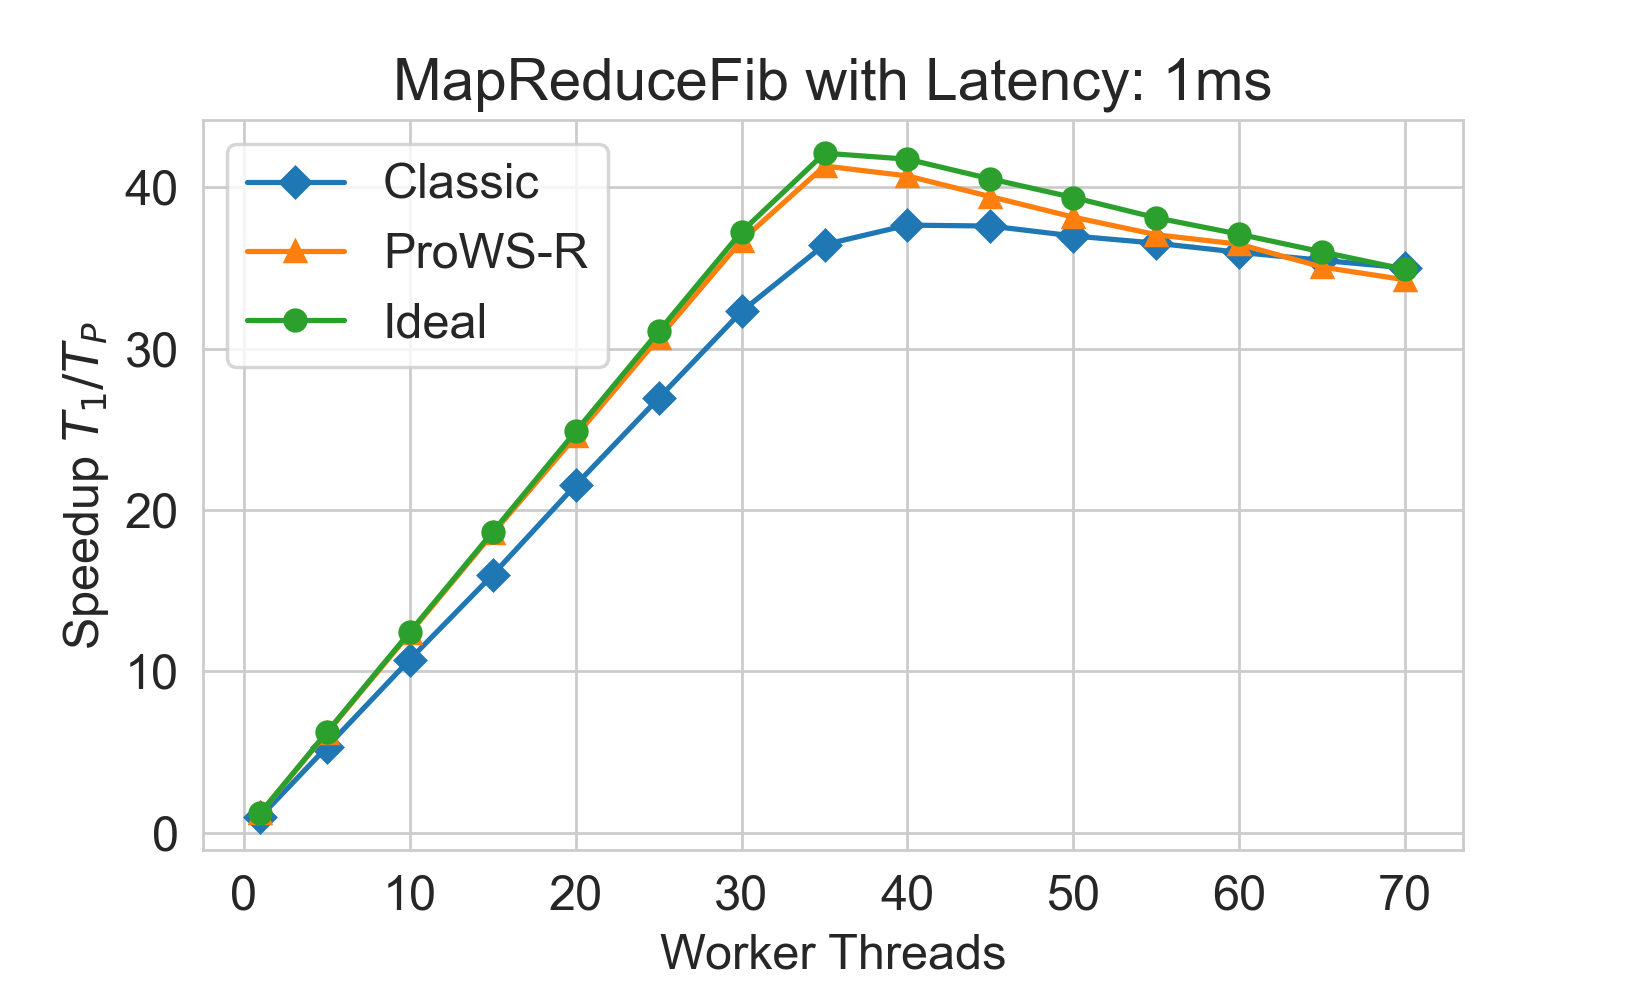
\includegraphics[width=0.8\linewidth]{figures/map_reduce_plot_latency_1.png}
    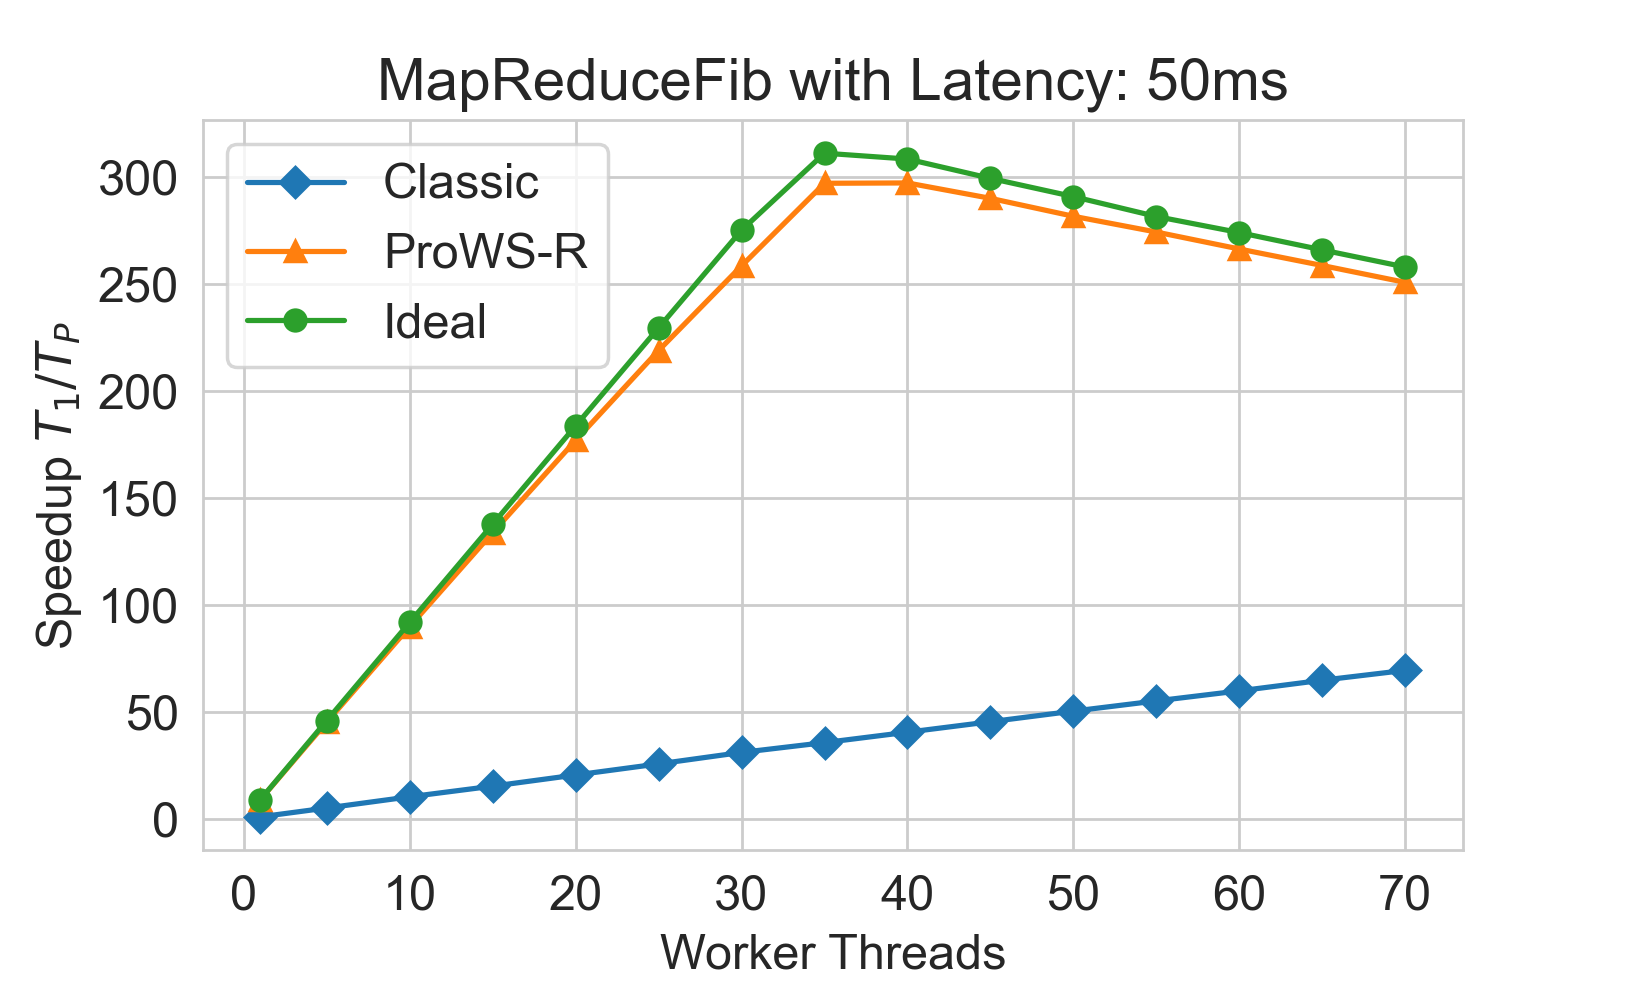
\includegraphics[width=0.8\linewidth]{figures/map_reduce_plot_latency_50.png}
    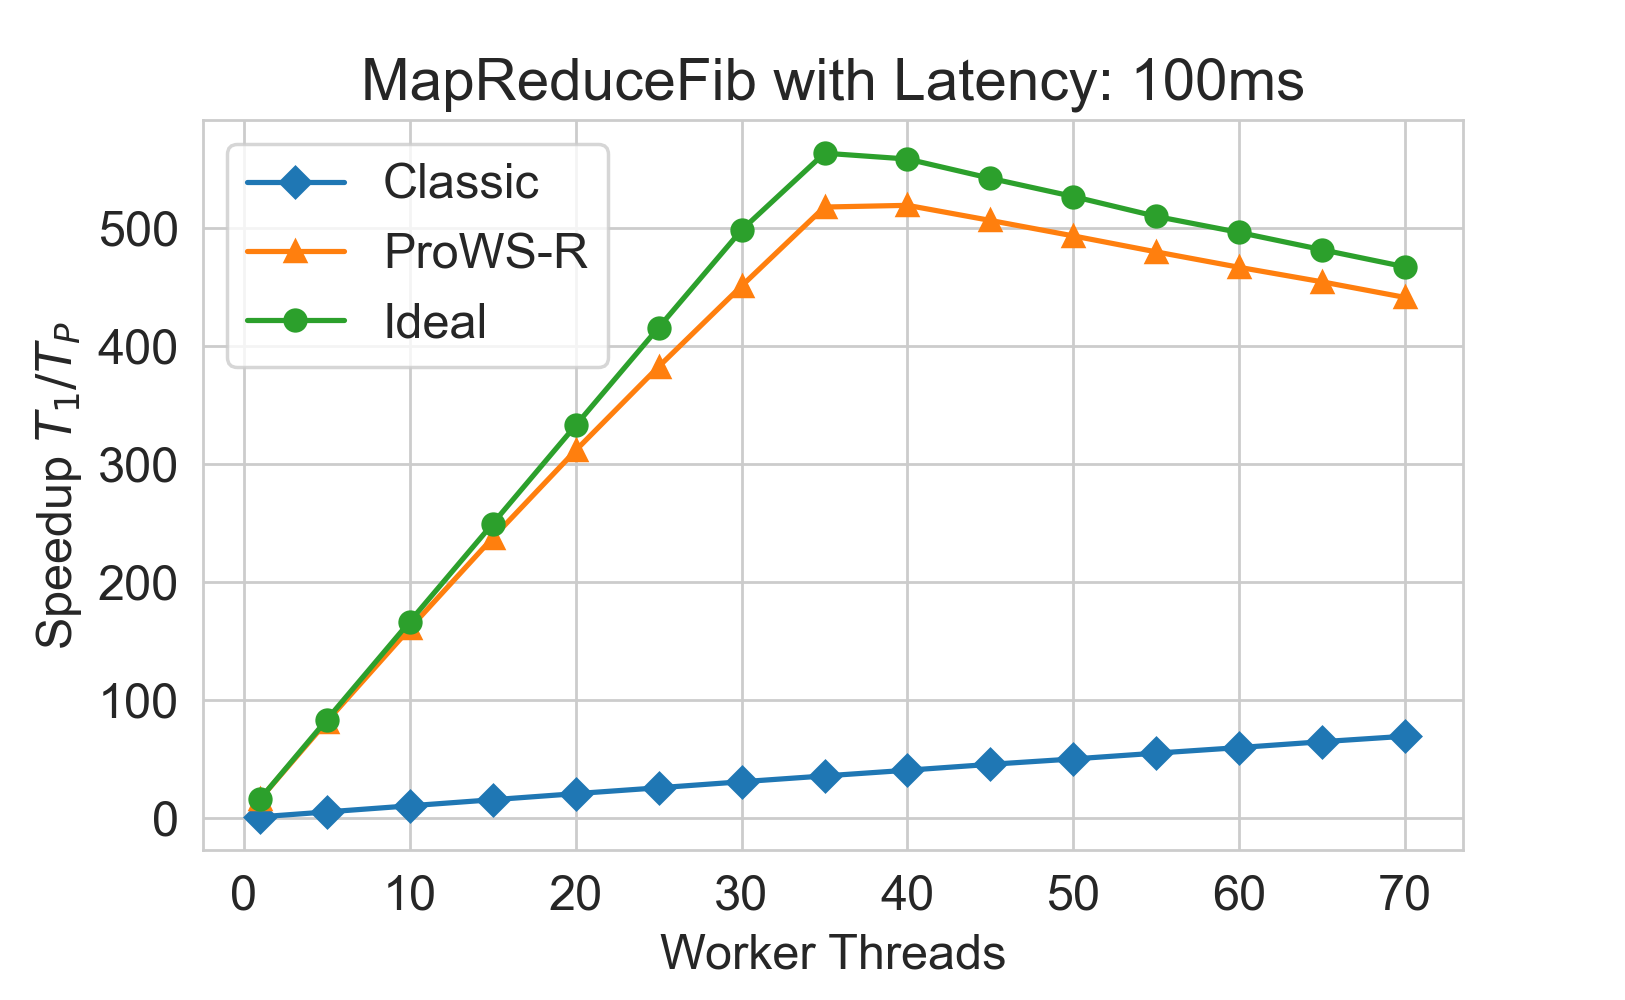
\includegraphics[width=0.8\linewidth]{figures/map_reduce_plot_latency_100.png}
    \caption{MapReduceFib benchmark results with varying latencies}
    \label{fig:map_reduce_plots}
\end{figure}

\section{Compute vs I/O Bound Workloads}
\label{section:compute_vs_i/o_bound_workloads}

This section seeks to answer the question of varying the ratio of compute vs I/O
bound operations in the workload. Whereas section
\ref{section:latency-hiding_efficiency} is concerned about the effects of
\textit{injecting} latency by keeping \(T_1\) constant and only varying the
amount of latency \(T_\text{latency}\), this section is interested in what
happens when the \textit{sum} of total work and latency \(T_1 +
T_\text{latency}\) is held constant but the individual parameters adjusted. In
other words, how does ProWS-R perform under workloads of varying natures?

This parameter sweep benchmark runs the naive recursive parallel Fibonacci
computation with a serial base case of zero, with the number of worker threads
set to the number of physical cores. When the computation hits the Fibonacci
base case (the leaf nodes in the computation DAG), it incurs latency by either
performing a blocking sleep to simulate a compute bound operation (a compute
bound operation \textit{must} take up processor cycles, there is no hiding
possible) or uses a future that suspends for the equivalent duration (but this
latency can be hidden). The percentage of I/O bound nodes in the workload
dictate whether the blocking sleep call or future will be used.

A plot showing the parameter sweep benchmark results is shown in figure
\ref{fig:param_sweep}. As expected, the greatest speedups come from when the
workload consists of a high percentage of I/O bound nodes. Speedup is also
increased when longer latency values are used, but not to the extent that the
I/O bound node percentage does. Essentially, when there is an abundance of
latency-hiding operations, the classic scheduler suffers tremendously as it must
bears the cost of each individual latency penalty, while ProWS-R can efficiently
hide this.

From this it is clear that the workloads that will benefit most from
latency-hiding are ones with a high percentage of latency-incurring operations,
and compute-bound workloads benefit less. Fortunately, in all cases, even when
the workload is purely compute-bound, ProWS-R performs better or equal to
classic work-stealing (a benchmark dedicated to compute-bound comparison is
discussed in section \ref{section:rayon-lh_scheduler_overhead}).

\begin{figure}[ht]
    \centering
    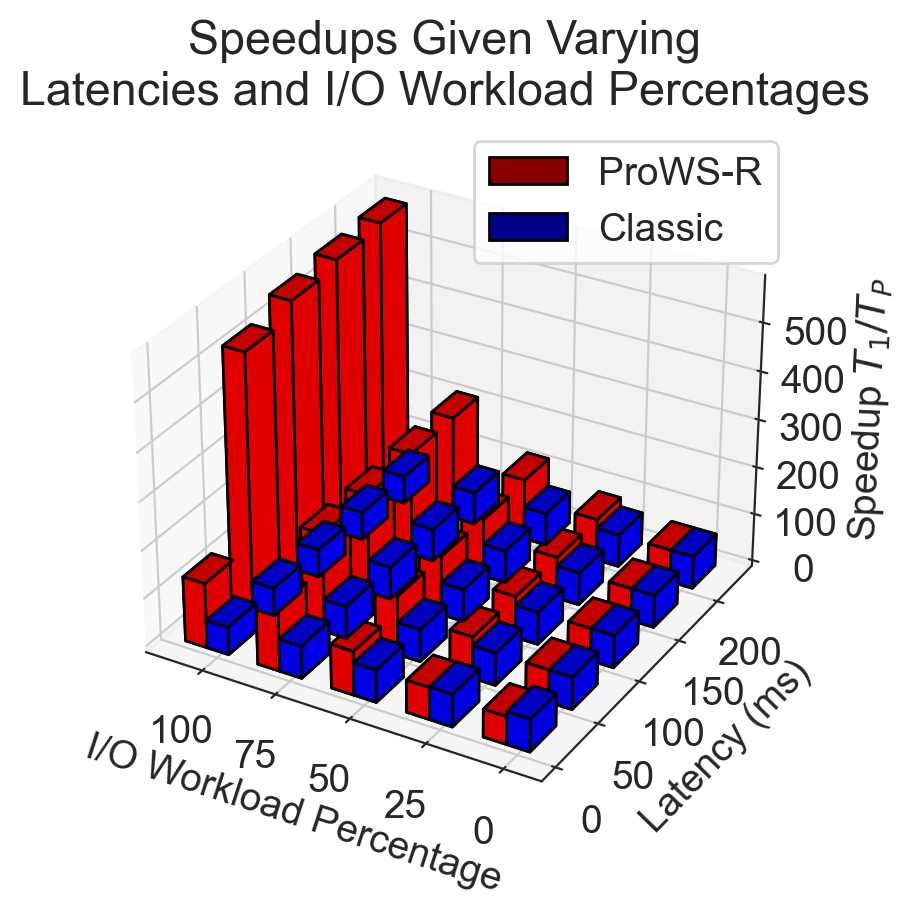
\includegraphics[width=0.6\textwidth]{figures/param_sweep_plot.png}
    \caption{Parameter sweep benchmark results}
    \label{fig:param_sweep}
\end{figure}

\section{Rayon-LH Scheduler Overhead}
\label{section:rayon-lh_scheduler_overhead}

While latency-hiding capabilities are great, it would be less than ideal if this
came at the cost of sacrificing performance on regular compute-bound workloads.

\section{Insights and Limitations}
\label{section:insights_and_limitations}

TODO: move concurrency difficulties here, talk about pinning, stack overflow,
tied to async-io

%%%%%%%%%%%%%%%%%%%%%%%%%%%%%%%%%%%%%%%%%%%%%%%%%%%%%%%%%%%%%%%%%%%%%%%%%%%%%%%%

\chapter{Conclusion: Patience Is Not a Virtue}

\section{Summary}

\section{Lessons Learned}

\section{Future Work}

\bibliographystyle{plain} \bibliography{references}

%% You can include appendices like this:
% \appendix
%
% \chapter{First appendix}
%
% \section{First section}
%
% Markers do not have to consider appendices. Make sure that your contributions
% are made clear in the main body of the dissertation (within the page limit).

\end{document}
